\documentclass[12pt,a4paper]{report} % ,twoside,openright

\usepackage[utf8]{inputenc}
\usepackage{graphicx}
\usepackage{hyperref}
\usepackage{fancyhdr}
\usepackage{listings}
\usepackage{color}
\usepackage{url}
\makeatletter
\g@addto@macro{\UrlBreaks}{\UrlOrds}
\makeatother

\linespread{1.5}

\definecolor{dkgreen}{rgb}{0,0.6,0}
\definecolor{gray}{rgb}{0.5,0.5,0.5}
\definecolor{mauve}{rgb}{0.58,0,0.82}
\definecolor{light-gray}{gray}{0.95}
\definecolor{yellow}{RGB}{255, 251, 140}

% defining single line code blocks with monospace font and light-gray backgound (StackOverflow style)
\newcommand{\code}[1]{\nolinkurl{#1}}
% note command
\newcommand{\todo}[1]{\colorbox{yellow}{\textbf{\#TODO} #1}}
% chapter -> capitolo
\renewcommand{\chaptername}{Capitolo}
% command for title pages
\newcommand{\doctitle}[2]{
\vspace*{3cm}
\begin{flushright}
\Large \textit{Documentazione a cura di\\#1}\\
\large (\texttt{#2})
\end{flushright}
\newpage
}

\begin{document}

\begin{titlepage}
\begin{center}

\includegraphics[width=\textwidth]{polimi_logo.jpg}
\Huge
\textbf{Progetto Giocoso 2015}

Documentazione delle Applicazioni

\vspace{5cm}
\normalsize
\textit{Ultimo aggiornamento: \today}
\end{center}
\end{titlepage}


\tableofcontents
\pagenumbering{arabic}
\setcounter{page}{1}

\chapter{Chef per un Giorno}
\newcommand*{\mypath}{chefperungiorno}%
\graphicspath{ {\mypath/images/} }

\doctitle{Giovanni Quattrocchi}{giovanni.quattrocchi@polimi.it}

\begin{figure}[h!]
\centering
\centering{
\includegraphics[width=\textwidth]{title.png}}
\end{figure}

\section{Design dell'Applicazione}
\subsection{Diagramma delle classi del modello}

Le classi del modello sono le seguenti:
\begin{description}
\item[Game] classe statica che permette il caricamento dei dati di gioca da JSON e mantiene una referenza ai livelli e ai piatti

\item[Level] classe astratta, il metodo getNumberOfIngredientForDish ritorna il numero corretto di elementi solo per il Livello 1

\item[Dish] il piatto, un insieme di ingredienti

\item[Ingredient] l’ingrediente

\item[Turn] tiene traccia del completamento di un piatto, invia callback al relativo TurnListener. Al termine del piatto genera un TurnResult.

\item[TurnListener] interfaccia per la ricezioni di eventi relativi a un turno

\item[TurnResult] il risultato del turno
\end{description}

\begin{figure}[h!]
\label{fig:uml}
\centering
\centering{
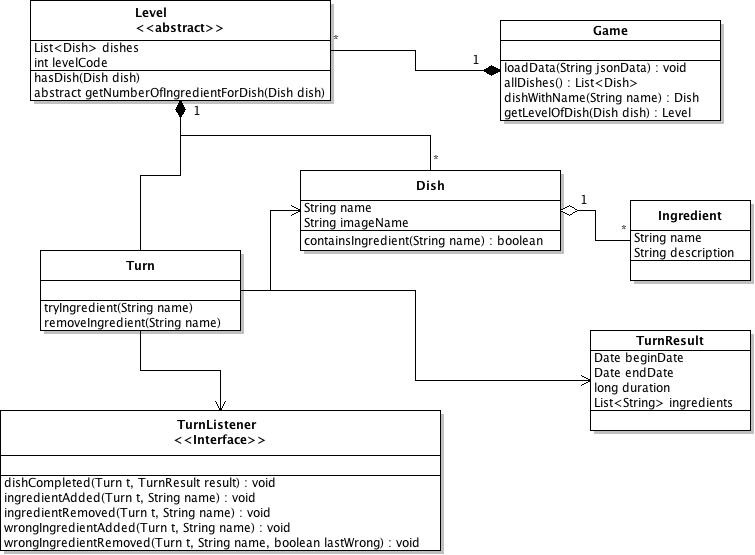
\includegraphics[width=\textwidth]{uml-class.jpg}}
\caption{Class Diagram}
\end{figure}

\subsection{AllJoyn}
La modalità multiplayer è stata realizzata attraverso AllJoyn. Qui si può trovare la documentazione completa: \url{https://allseenalliance.org/developers/develop/api-guide/core/android}.
L’applicazione espone un generico MultiPlayerService con il metodo \code{sendMessage()}. Questo metodo permette di inviare semplici Signal con un parametro stringa.
Il formato di invio dei messaggi è CSV, il primo elemento è il tipo del messaggio.
Verranno inviati tre tipi di messaggi:
\begin{enumerate}
\item dishes seguito dai nomi del piatti, rappresenta l’inizio del gioco, l’host della partita invia al joiner della sessione i piatti selezionati
\item stop inviato quando uno dei due dispositivi abbondona il gioco (alla ricezione di questo messaggio si torna indietro alla schermata principale)
\item dish seguito dal nome del piatto, indica il completamento di un piatto
\end{enumerate}

\subsection{Gimbal}
Nel gioco ciascun ingrediente è un trasmettitore Gimbal. Nell’applicazione si fa uso della versione 2 dell’API, in particolare si fa uso della parte di Beacon management. Qui la documentazione: \url{https://gimbal.com/doc/android/v2/devguide.html\#set\_beacon}
Tale API viene utilizzata nella MainActivity per orchestrare il flow del gioco. I beacon sono associati ad un ingrediente attraverso il name. La vicinanza di un beacon è determinata dal valore del suo RSSI. Il valore che discrimina la vicinanza di un beacon è -60. Attenzione: potrebbe essere necessario cambiare il threshold di vicinanza (si trova nella classe \code{Commons.java}).


\subsection{Activities}

L’applicazione dispone di quattro Activity:
\begin{description}
\item[StartActivity] mostra la schermata principale e carica i dati del gioco per evitare successivi caricamenti. Dispone di un bottone per l’inserimento della email per l’invio delle statistiche del gioco. La persistenza della email è affidata alle SharedPreferences di Android

\item[ChooseSessionActivity] mostra la schermata di scelta dei piatti, cerca nell’Intent un Extra “mode” che indica la modalità di gioco (singola o multiplayer). La selezione dei piatti può avvenire in due modi: selezionandoli da una GridView o premendo il tasto “Casuale”

\item[MultiPlayerConfigActivity] gestisce parte dall’inizializzazione della logica di AllJoyn, il comportamento varia a seconda se il giocatore seleziona di creare una partita (ruolo host) o di accedere ad una partita (ruolo joiner)

\item[MainActivity] orchestra la partita usando Gimbal API, AllJoyn Framework, la classe \code{Turn} e \code{TurnListener}. Cerca nell’Intent un Extra “mode” per la modalità e uno “dishes” per i piatti. 
\end{description}

Di seguito viene riportato il flow di accesso alle diverse activity.

\begin{figure}[h!]
\label{fig:flow}
\centering
\centering{
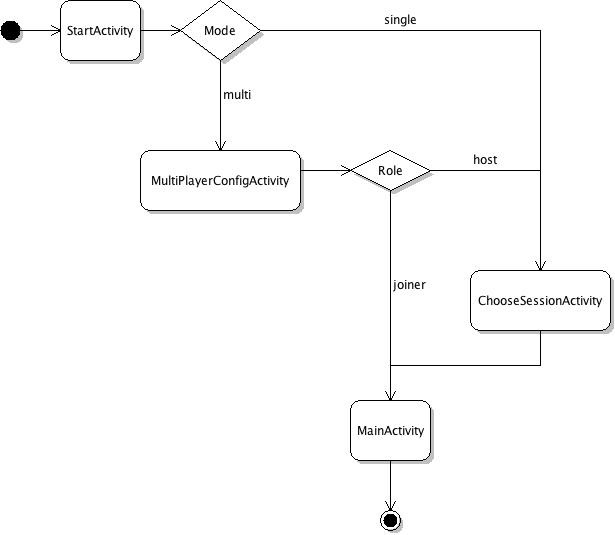
\includegraphics[width=\textwidth]{uml-activity1.jpg}}
\caption{Flow di accesso alle activity}
\end{figure}


Durante una partita il tasto Back di Android riporta alla schermata iniziale dopo una conferma. Nel caso di Multiplayer se un dispositivo abbandona la partita anche l’altro torna alla schermata principale.


\subsection{Adapters}

Per visualizzare liste di oggetti sono stati usati i seguenti Adapter:
\begin{description}
\item[DishAdapter] viene utilizzato nella schermata di selezione dei piatti, tiene traccia degli elementi selezionati

\item[IngredientAdapter] controlla la visualizzazione delle interazioni tra ingredienti e dispositivo. Mostra immagini diverse a seconda dell’assenza di ingredienti, ingredienti presenti o errati

\item[TableAdapter] controlla la visualizzazione della tavola con i sottopiatti vuoti o riempiti da quelli completati dalla squadra relativa al dispositivo e anche dalla squadra avversaria in caso di multiplayer.
\end{description}

Altre classi e file
\begin{description}
\item[Commons] contiene costanti, della logica condivisa durante il gioco (AllJoyn) e metodi statici (invio mail)

\item[GMailSender] e JSSEProvider classi helper per l’invio di email

\item[PrefUtils] classe helper per la gestione delle SharedPreferences

\item[\code{/raw/data.json}] file contente i dati del gioco (ingredienti, livelli, piatti)

\item[\code{/raw/data\_source.csv}] file originale in csv in cui erano contenuti i dati del gioco non ben strutturati

\item[\code{/raw/gen\_json.py}] script python per trasformare \code{data\_source.csv} in \code{data.json}
\end{description}


\section{Manuale di Istruzioni}
\subsection{Introduzione}
Chef per Un Giorno è un gioco per dispositivi Android. Lo scopo del gioco è indovinare gli ingredienti necessari per la preparazione di un piatto attraverso l’avvicinamento di trasmettitori Gimbal al dispositivo. Sono supportate due modalità: modalità singola (una squadra) e modalità multipla (due squadre).

\textbf{ATTENZIONE}: per il corretto funzionamento dell’applicazione è necessario attivare sia il Wi-Fi sia il Bluetooth.

\subsection{Preparazione}

Per giocare è necessario configurare i trasmettitori Gimbal. Le credenziali d’accesso al portale Gimbal (\url{https://manager.gimbal.com}) verrano fornite su richiesta scrivendo una email a giovanni.quattrocchi@polimi.it.

\begin{enumerate}
\item Entrare nel portale Gimbal all’indirizzo \url{https://manager.gimbal.com}
\item Selezionare nella barra laterale Beacons (vedi figura \ref{fig:beacons})

\begin{figure}[h!]
\centering{
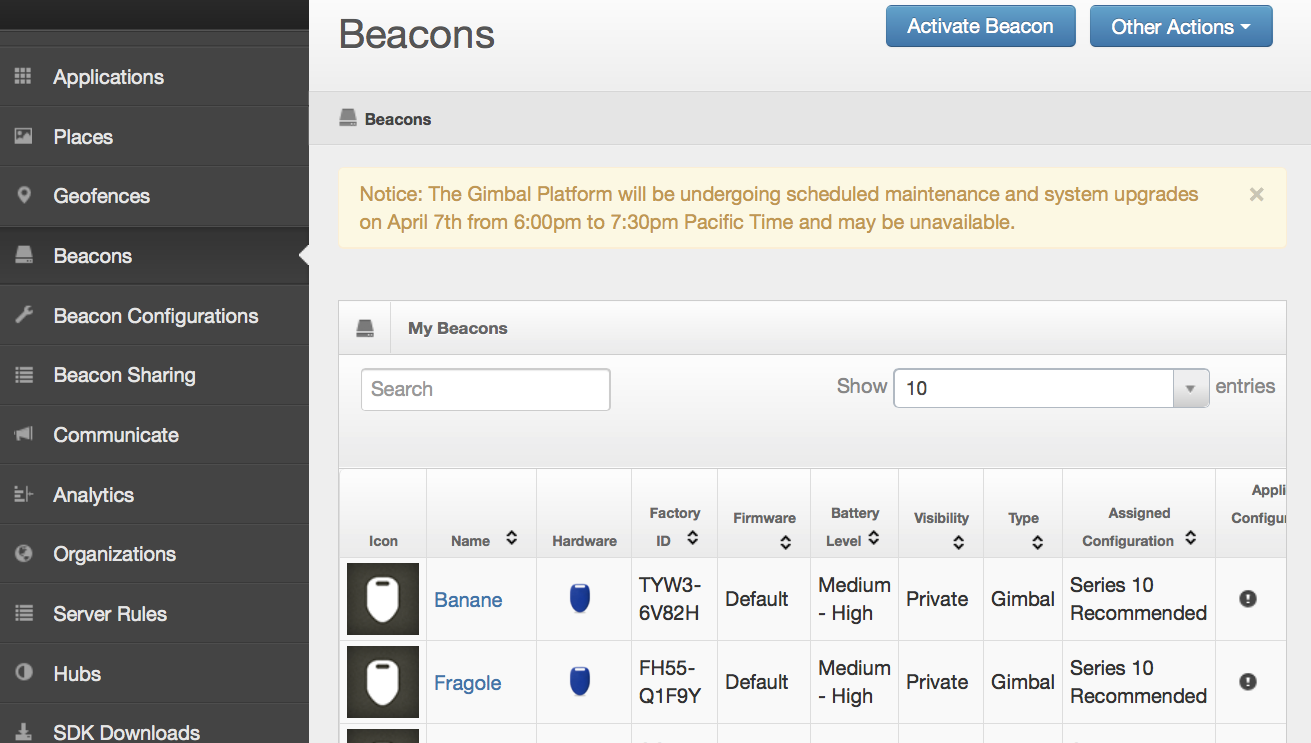
\includegraphics[width=\textwidth]{beacons.png}}
\caption{La schermata contenente il listato dei beacon nel portale Gimbal}
\label{fig:beacons}
\end{figure}

\item Selezionare il bottone Activate Beacon
\item Aprire un trasmettitore Gimbal e trovare il Factory ID (per come trovare il Factory ID, vedi figura \ref{fig:factoryid})

\begin{figure}[h!]
\centering{
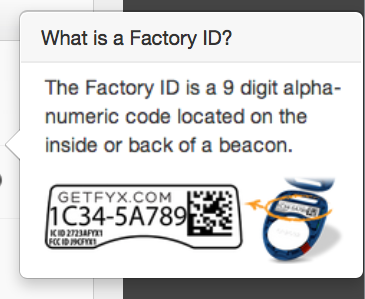
\includegraphics[width=\textwidth]{factoryid.png}}
\caption{Il factory ID di un beacon}
\label{fig:factoryid}
\end{figure}

\item Inserire come nome del Beacon l’ingrediente esattamente come riportato nell’ElencoIngredienti (fornito di seguito) e il Factory ID (vedi figura \ref{fig:activate-beacon})

\begin{figure}[h!]
\centering{
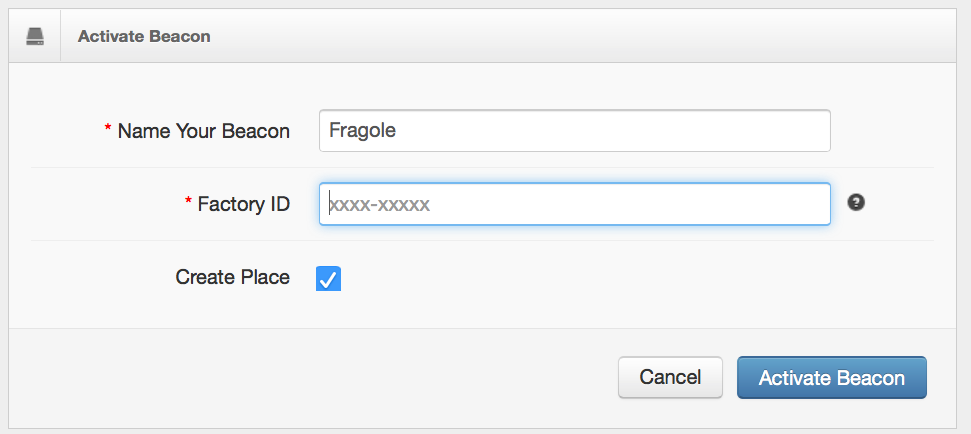
\includegraphics[width=\textwidth]{activate-beacon.png}}
\caption{Schermata di attivazione di un beacon nel portale Gimbal}
\label{fig:activate-beacon}
\end{figure}

\item Confermare con Activate Beacon
\item Ripetere per tutti i trasmettiri/ingredienti
\end{enumerate}

\subsection{Elenco Ingredienti}
\begin{itemize}
\item Ciliegie
\item Mirtilli
\item Uova
\item Pomodori
\item Insalata verde
\item Piselli
\item Zucchero
\item Zucchine
\item Banane
\item Gamberi
\item Mele
\item Kiwi
\item Riso
\item Fagioli
\item Farina
\item Latte
\item Peperoni
\item Pasta
\item Mozzarella
\item Fragole
\item Mango
\item Carote
\item Pollo
\item Ceci
\item Cetrioli
\item Cipolle
\end{itemize}

\subsection{Il gioco}
\subsubsection{Schermata Iniziale e principi generali}

\begin{figure}[h!]
\centering{
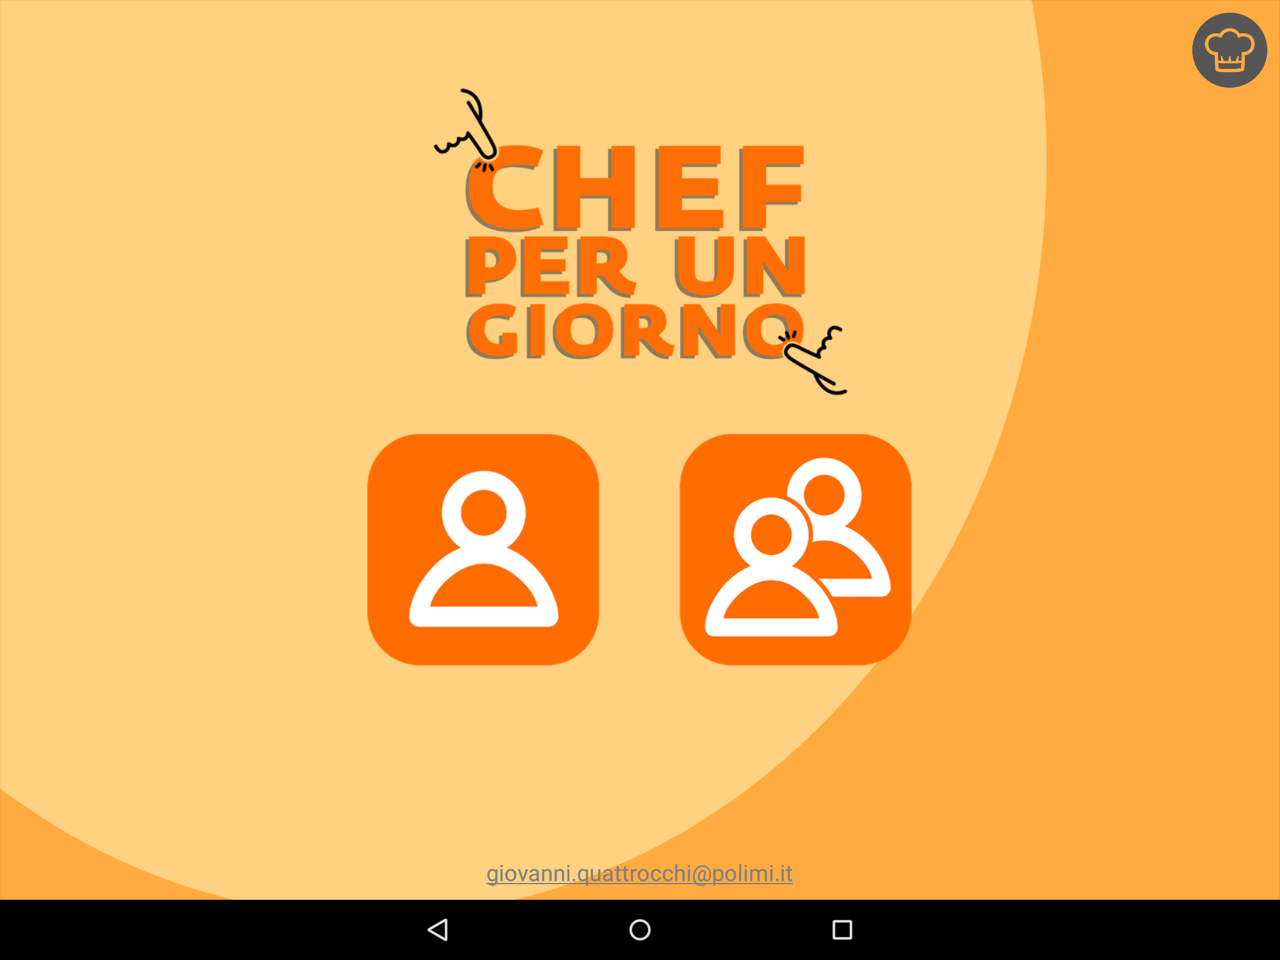
\includegraphics[width=\textwidth]{splash.png}}
\caption{Lo splash screen di Chef per un Giorno}
\label{fig:splash}
\end{figure}

La prima schermata (vedi figura \ref{fig:splash}) permette di scegliere tra la modalità singola o multipla. In basso al centro della schermata è anche possibile inserire un indirizzo mail per l’invio dei dati di gioco. Per tornare indietro a questa schermata dalla altre è necessario selezionare il pulsante indietro nella barra inferiore (indicato con un triangolo orientato verso sinistra). 
Il tavolo di gioco comprende il dispositivo Android e uno spazio dove appoggiare i trasmettitori.
Prima di preparare qualsiasi piatto allontanare tutti i trasmettitori dal tavolo di gioco.

\subsubsection{Modalità Singola}

Se si seleziona modalità singola comparirà la schermata di selezione dei piatti (vedi figura \ref{fig:screen1}). È possibile scegliere due o quattro piatti da preparare. Dopo averli selezionati cliccare il tasto Ok per continuare. In alternativa è possibile generale una partita con piatti casuali (è casuale anche il numero di piatti) schiacciando il tasto Casuale.
Dopo la scelta dei piatti comparirà la schermata di gioco principale (vedi figura \ref{fig:screen2}). A sinistra in alto comparirà il piatto da preparare, sotto di questo, se il piatto appartiene al Livello 1, appariranno anche tante pentole arancioni quanti sono il numero degli ingredienti. Se il piatto appartiene al Livello 2 non comparirà nulla. 
Avvicinando un trasmettitore al tavolo di gioco comparirà una pentola verde se l’ingrediente appartiene al piatto, rossa se non appartiene. La pentola rossa indica che c’è almeno un ingrediente errato (possono essere anche due, tre, e così via) e scomparirà quando tutti gli ingredienti errati saranno allontanati dal tavolo di gioco. Un piatto è completato quando vengono avvicinati tutti gli ingredienti corretti e nessuno errato.
Una volta completato il piatto, questo verrà aggiunto alla tavola e verrà mostrato il nuovo piatto da preparare. Quando tutti i piatti sono preparati il gioco è terminato. Per tornare alla schermata principale cliccare il tasto indietro di Android.

\begin{figure}[h!]
\centering{
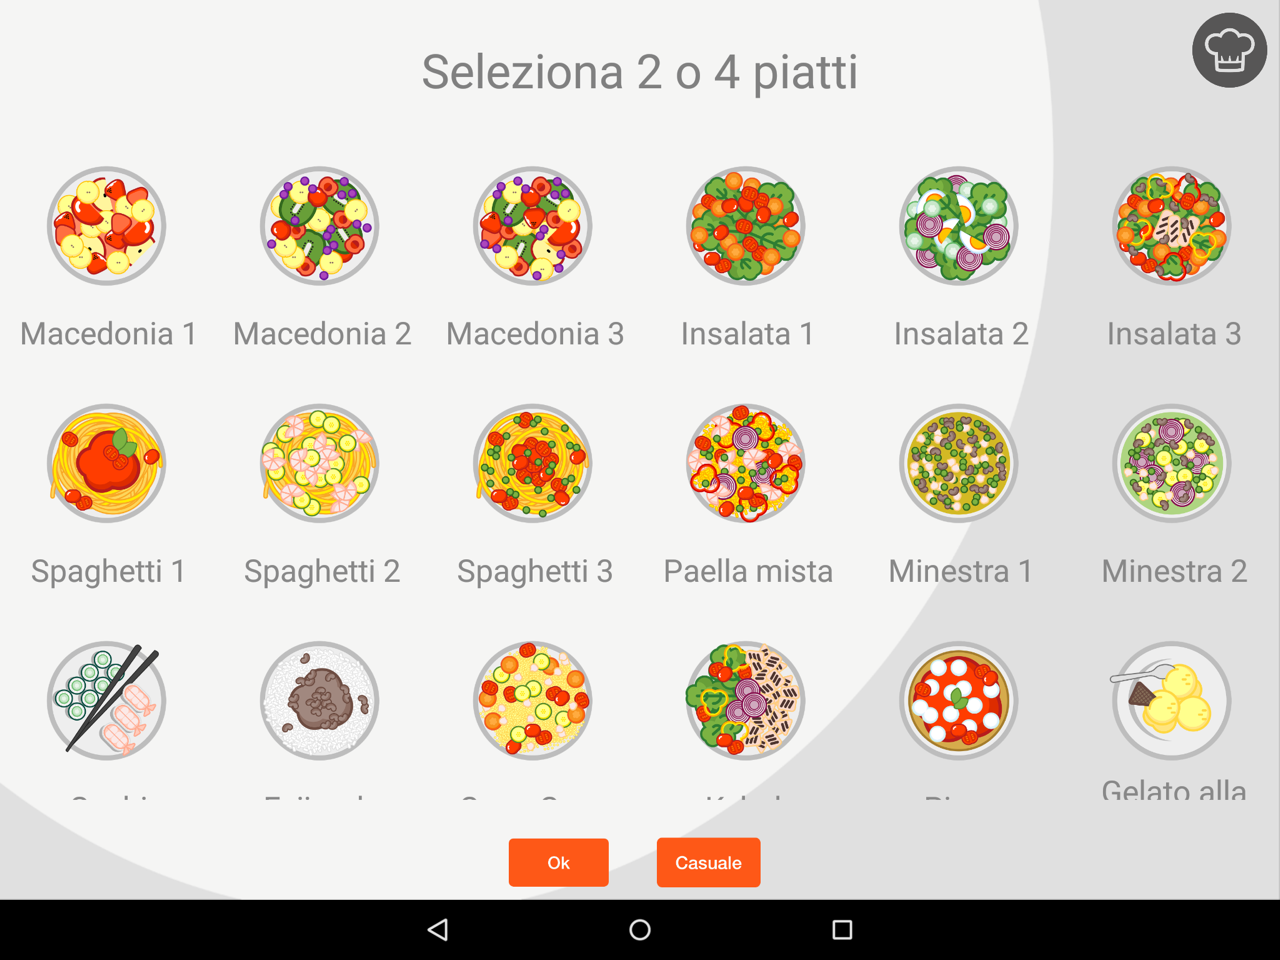
\includegraphics[width=\textwidth]{screen1.png}}
\caption{La schermata di selezione dei piatti}
\label{fig:screen1}
\end{figure}

\begin{figure}[h!]
\centering{
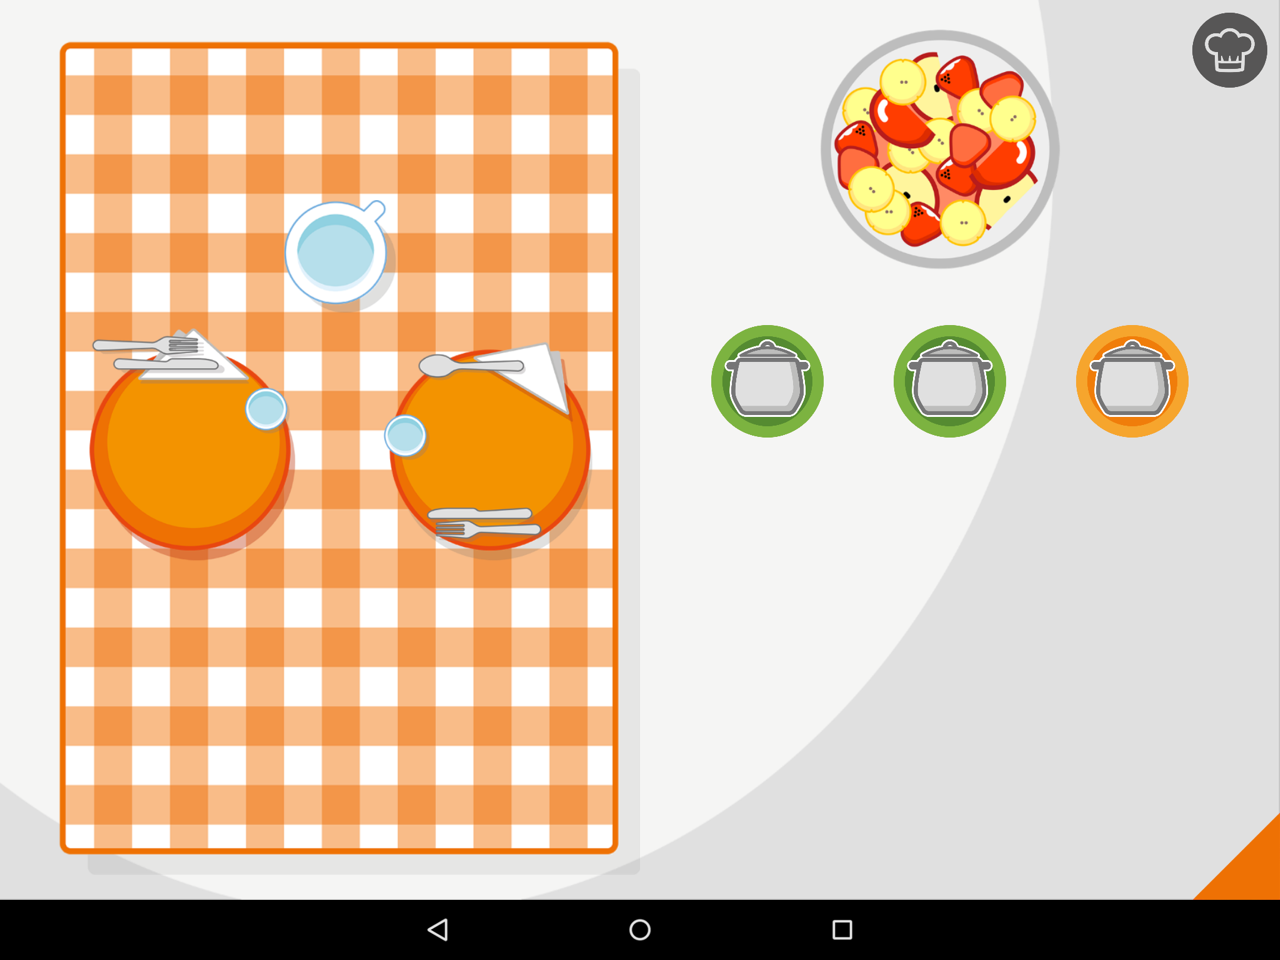
\includegraphics[width=\textwidth]{screen2.png}}
\caption{La schermata di gioco in modalità single player}
\label{fig:screen2}
\end{figure}


\subsubsection{Modalità Multiplayer}
È molto simile alla modalità singola con le seguenti varianti:
\begin{itemize}
\item I due dispositivi devono essere connessi alla stessa rete Wi-Fi
\item I due tavoli di gioco devono essere lontani l’uno dall’altro per evitare interferenze
\item Prima della selezione dei piatti è necessario che su un dispositivo si selezioni Crea una partita e sull’altro Entra in una partita
\item È obbligatorio selezionare quattro piatti (2 per squadra)
\item I quattro piatti verrano scelti dal dispositivo che crea la partita, l’altro rimarrà in attesa fino a selezione avvenuta
\item Giocano due squadre quella arancione e quella viola, il colore della squadra è indicato nella schermata di gioco dal colore presente nell’angolo in basso a destra.
\item Quando un piatto è completato da una squadra, questo compare anche nella tavola della squadra avversaria
\item Se su uno dei due dispositivi esce dal gioco, anche l’altro abbandonerà il gioco
\end{itemize}
In figura \ref{fig:screen3} è mostrata la schermata di gioco in modalità multiplayer.

\begin{figure}[h!]
\centering{
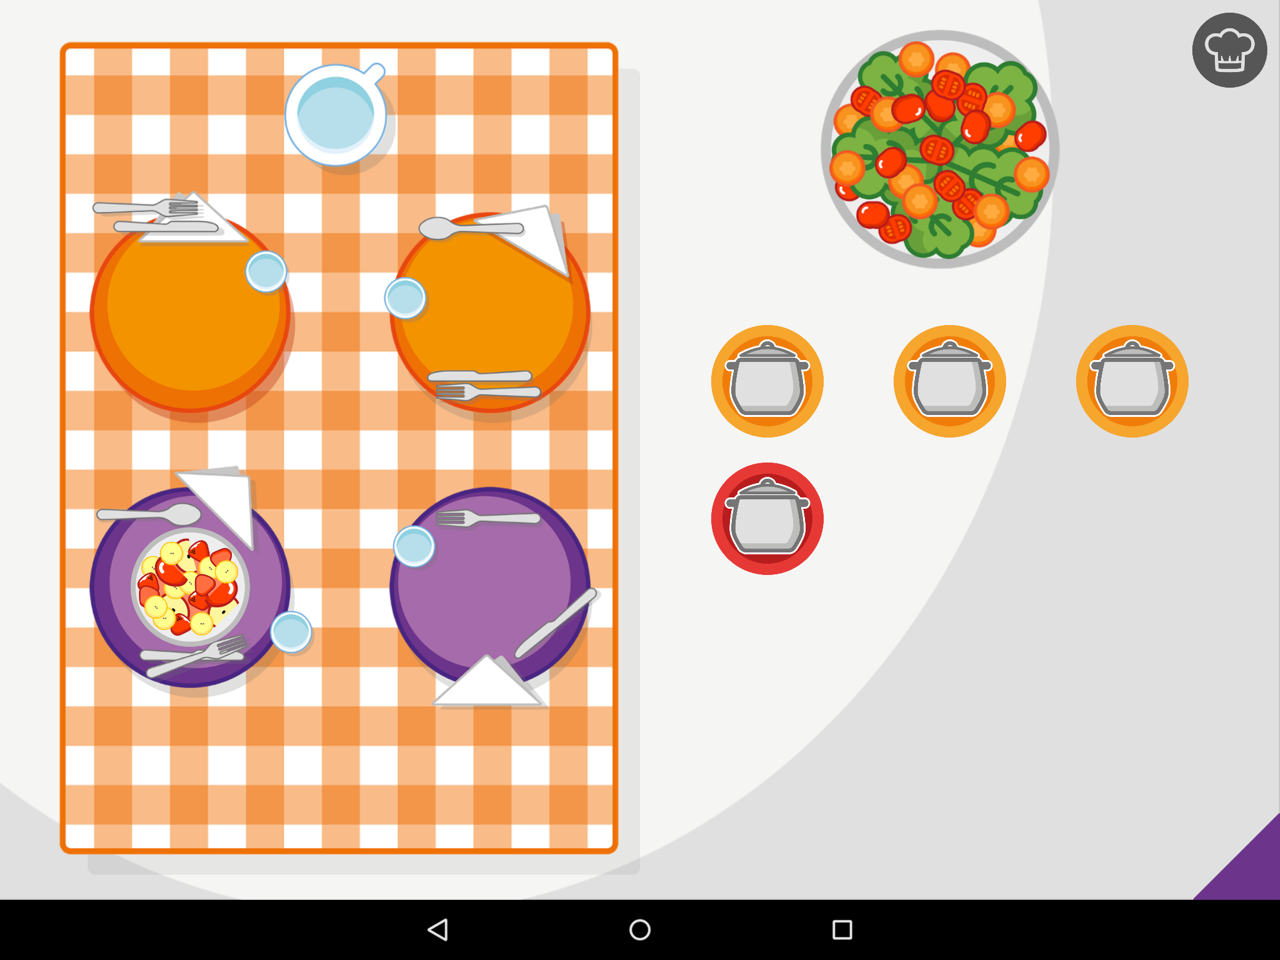
\includegraphics[width=\textwidth]{screen3.png}}
\caption{La schermata di gioco in modalità multiplayer}
\label{fig:screen3}
\end{figure}

\subsubsection{Invio dei dati di gioco}

Se è stata inserita una mail valida (vedi Schermata Principale) verrà inviata una mail con i seguenti dati per ogni piatto realizzato:

\textless nome del piatto\textgreater, \textless timestamp inizio\textgreater, \textless timestamp fine\textgreater, \textless durata in secondi\textgreater, \textless ingredienti in ordine di rilevazione\textgreater, \textless errori\textgreater

Es:

Macedonia 1, 1428877207567, 1428877307567, 100, Mele, Fragole, Banane, errors(Carote, Pomodori)



\chapter{Lego Digital Sonoro 1}
\renewcommand*{\mypath}{legodigitalsonoro1}%
\graphicspath{{\mypath/images/}}

\doctitle{Chiara Calabrese}{chiara.calabrese@mail.polimi.it}

\newcommand{\includefigure}[2]{
\begin{figure}[h!]
\centering{
\includegraphics[width=\textwidth]{#1.png}}
\caption{#2}
\label{fig:#1}
\end{figure}
}

\section{LegoDigitalSonoro: istruzioni d'uso}

L'applicazione LegoDigitalSonoro è una applicazione mobile progettata per la compatibilità con Android. L'applicazione è un semplice gioco dedicato ai bambini in età prescolare il cui intento è quello di insegnare loro a comporre delle parole bisillabe.

Al giocatore vengono presentate 4 o 6 tessere rappresentanti una sillaba di una determinata parola. Ogni tessera è associata ad una seconda tessera con cui andrà a formare una parola bisillaba. Ad ogni parola è associata una rappresentazione, quindi per esempio alla parola "cane" sarà associata la figura di un cane, alla parola "mora" una mora e così via. Ogni immagine è divisa a metà in due tessere rappresentanti le due sillabe componenti la parola. Il gioco consiste nel selezionare la coppia di tessere nella successione corretta per formare una parola di senso compiuto. Una volta accoppiate tutte le tessere della schermata il gioco sarà completato. L'applicazione raccoglie dati sulla velocità con cui il bambino compone una determinata parola e li invia via mail ad un indirizzo prescelto.

L'applicazione è composta da poche semplici schermate. Nella prima schermata è possibile scegliere di iniziare una partita in modalità singola o in modalità sfida, se si vuole giocare con un altro giocatore. Da questa schermata è possibile accedere ad un'altra detta "di configurazione" che permette di modificare le impostazioni di gioco selezionando il numero di parole componibili in una schermata o turno, 2 o 3, il numero di turni di gioco, da 1 a 10, e l'indirizzo mail a cui inviare i risultati alla fine della partita. Le impostazioni predefinite per il numero di turni è 8, per il numero di parole per turno è 3 e per la mail è il campo vuoto.

\includefigure{main}{Schermata iniziale}

\includefigure{impostazioni}{Schermata impostazioni}

Selezionando la modalità gioco singolo, l'utente accede direttamente alla schermata di gioco. Questa schermata è divisa in due settori principali ovvero una sezione a sinistra, che presenta 3 tessere vuote, e una sezione a destra, con le tessere delle parole da comporre. Per comporre le parole l'utente selezionerà le sillabe cliccando sopra ciascuna tessera. Quando si seleziona una tessera si può ascoltare il suono della sillaba associata. Le parole devono essere composte nell'ordine corretto, prima-sillaba seconda-si llaba. Se l'utente seleziona per prima una prima sillaba questa comincia a lampeggiare, indicando univocamente quale parola deve essere completata. Se l'utente seleziona correttamente la seconda sillaba la parola è completata e si sposta nella parte sinistra dello schermo, altrimenti la prima sillaba continua a lampeggiare. Ogni volta che una tessera viene selezionata viene pronunciata la sillaba corrispondente.

Al momento in cui la parola viene completata l'applicazione pronuncia la parola completa. L'utente la può riascoltare selezionando la tessera nel campo risultati, oppure può selezionare la bandiera inglese accanto alla stessa tessera che permette di ascoltare la stessa parola in inglese.

Quando il giocatore completa tutte le parole, ovvero quando la parte sinistra dello schermo è completa, sulla parte destra comparirà un bottone che permette di passare al turno successivo o, se le parole sono state tutte completate, permette di terminare la partita. Una volta terminata la partita l'applicazione riporta l'utente alla schermata iniziale.

\includefigure{gioco}{Schermata di gioco}

Se viene selezionata la modalità di gioco "sfida", si accede invece ad una schermata di impostazione della connessione. La connessione con altri giocatori avviene tramite bluetooth.

Accedendo alla schermata di impostazioni della partita doppia verrà richiesto all'utente il permesso di rendersi visibile agli altri dispositivi per 5 minuti. I dispositivi con cui possiamo interagire si dividono in due categorie: la prima è formata dai dispositivi con cui ci siamo connessi già in passato, la seconda da quei dispositivi con cui non abbiamo mai interagito. Dando il permesso alla richiesta del sistema, ci si rende visibili a quei dispositivi con cui non abbiamo mai parlato; è quindi una operazione fondamenta le quando dobbiamo instaurare una connessione con un giocatore per la prima volta.

Perchè due giocatori possano giocare insieme occorre che entrambi selezionino la modalità di gioco sfida. Una volta che entrambi hanno raggiunto la schermata di impostazioni della partita doppia uno dei due invita il secondo a giocare. Cliccando il bottone centrale si ha accesso alla lista di dispositivi riconosci uti. Se la lista è vuota o l'altro giocatore non compare nella lista basterà cliccare sul bottone "scan" per dare avvio alla ricerca di nuovi dispositivi. Una volta che l'altro giocatore compare nella lista di possibili sfidanti, chi imposta la partita lo invita a giocare. A questo punto la partita doppia ha inizio, l'applicazione mostrerà la schermata di gioco ad entrambi i giocatori e l'invitato potrà eseguire la prima mossa. I turni sono alternati e indicati da un semaforo in basso a destra. La composizione delle parole è collaborativa, quindi il primo giocatore selezionerà la prima sillaba e il secondo dovrà completare la parola selezionat a e successivamente scegliere la prima sillaba della seconda parola. Il gioco continua fino all'esaurimento delle parole sullo schermo.

\includefigure{connectionsetup}{Schermata connection setup}

\includefigure{schermataDeviceList}{Schermata impostazione della partita doppia: lista dei giocatori disponibili}

L'applicazione LegoDigitalSonoro1 permette di raccogliere i dati sulla partita appena giocata. Ogni volta che viene completata una partita in modalità giocatore singolo, viene inviata una mail all'indirizzo specificato nelle impostazioni contenente il numero di parole totale, tutte le parole completate e, per ogni parola, il tempo di completamento.

\section{LegoDigitalSonoro: design}

L'applicazione LegoDigitalSonoro è stata progettata per girare su Android 4.2. I dati sono incorporati all'interno dell'applicazione, quindi non occorre scaricare da remoto alcuna informazione. L'unico contatto con un sistema remoto avviene al momento della inizializzazion e della partita in modalità "sfida".

L'applicazione è costituita da 3 activity principali che sono la \emph{MainActivity}, che controlla la schermata inziale e permette all'utente di scegliere fra partita singola, multipla o modifica delle impostazioni, la \emph{MatchActivity}, che controlla la schermata di gioco, e la \emph{ConnectionSetupActivity}, che gestisce la schermata di setup della partita in modalità doppio giocatore.

\includefigure{activities}{Diagramma delle Actvity}

I dati sono costituiti da un file \emph{txt} inserito nella cartella degli assets, che contiene su ogni riga l'informazione per una determinata parola. I dati sono composti da una stringa che contiene la parola in italiano, due stringhe, una per ciascuna sillaba, e una stringa che costituisce la traduzione in inglese della parola stessa. Il file viene letto una volta in fase di inizializzazione della partita. Altri dati sono costititi dalle immagini associate alle parole e dalle immagini relative a bottoni e agli altri elementi grafici, contenute nelle cartelle \emph{drawable}.

Per gestire il dato "parola" abbiamo creato il tipo di dato \emph{Word} di cui fanno parte una stringa per il nome, due istanze del tipo di dato \emph{Syllable} e una stringa per la traduzione della parola in inglese. La risorsa grafica associata alla parola è identificata dalla stringa della parola che rappresenta.

\includefigure{word}{Class diagram: Word e Syllable}

La partita è regolata dalla \emph{MatchActivity} che al momento della inizializzazione recupera le informazioni sulla partita dalle \emph{preferences} (numero di turni e numero di parole per turno), controlla la modalità di gioco (singola o sfida) e instanzia il \emph{MatchManager}. Il \emph{MatchManager} gestisce la logica della partita, inizializza il gioco e ne modifica lo stato in base all'input dell'utente. Il compito del \emph{MatchManager} in fase di inizializzazione è quello di instanziare il \emph{WordManager} che a sua volta instanzia un \emph{WordReader} per creare le parole e divide le parole nei diversi turni. La \emph{MatchActivity} possiede inoltre due fragment che controllano lo stato dei due settori di cui è composta l'interfaccia grafica. Un fragment è chiamato \emph{ResultFragment} e contiene le informazioni riguardanti le parole indovinate, l'altro è invece il \emph{PlaygroundFragment} che gestisce la griglia in cui sono inserite le tessere. Dato che il \emph{MatchManager} contiene le informazioni sullo stato della partita avrà un elenco per le parole presenti sulla schermata, uno per le sillabe nel fragment \emph{PlaygroundFragment} e uno per i risultati nel \emph{ResultFragment}. La \emph{MatchActivity} implementa l'interfaccia \emph{ResultCallback}, che permette di osservare le scelte dell'utente nel \emph{PlaygroundFragment} e modificare di conseguenza il \emph{ResultFragment}. 

\includefigure{architectureGiocoso}{Class Diagram: Classi per la gestione dello stato della partita}

\subsection{Partita singola}
Per inzializzare la partita singola il giocatore seleziona il bottone apposito nella \emph{MainActivity}. In questo modo viene chiamato il metodo \emph{startSingleMatch} che rimanda alla \emph{MatchActivity}.

Nel caso di partita singola l'inizializzazione prevede che le parole vengano lette dal file di testo e raccolte dal \emph{WordReader}. Il \emph{WordManager} seleziona un sottoinsieme casuale delle parole del \emph{WordReader} definito in base alle informazioni delle impostazioni (il numero di parole sarà pari al prodotto fra numero di turni e numero di parole per turno). Le parole sono poi raccolte in tanti sottoinsiemi quanti sono i turni.

\includefigure{initSingle}{Sequence Diagram: inizializzazione della partita gioco singolo}

Una volta inizializzata la partita sullo schermo del giocatore appare una schermata con due sezioni, ognuna gestita da un apposito fragment. Le tessere sono inserite in una \emph{GridView}, a cui è associato un \emph{GridAdapter}. Il \emph{PlaygroundFragment} viene aggiornato ogni volta che l'utente seleziona una delle tessere, e la tessera selezionata viene comunicata al \emph{MatchManager} che in base a questa informazione aggiorna lo stato del gioco.

Il \emph{MatchManager} in base alla tessera selezionata, ovvero alla sillaba, può avere diversi comportamenti. Se la sillaba selezionata non completa nessuna parola ma è la prima prima sillaba valida ad essere selezionata, viene aggiornata l'ultima parola valida, se la sillaba selezionata coincide con la seconda sillaba dell'ultima parola valida viene aggiornato l'elenco dei risultati e viene notificato il \emph{ResultFragment}, se la sillaba non è valida, ovvero è la prima ad essere selezionata ma non è la prima di una parola, o ancora non completa l'ultima parola valida, il \emph{MatchManager} non aggiorna nulla. Abbiamo scelto, in questo caso, di non aggiornare l'ultima parola valida se il giocatore seleziona una nuova prima sillaba dopo la prima sillaba valida registrata. In questo modo al giocatore sarà chiaro che per passare al completamento di una nuova parola è necessario completare la parola precedentemente iniziata.

\includefigure{onsyllselected}{Sequence Diagram: selezione della prima sillaba di una parola, in questo caso non verrà eseguita la parte nel riquadro opzionale dal momento che stiamo considerando la modalità di gioco singolo giocatore}

\includefigure{onsyllselected1}{Sequence Diagram: completamento di una parola}

Quando l'utente seleziona una tessera che completa la parola valida, il \emph{PlaygroundFragment} lo notifica al \emph{ResultFragment} che aggiorna il contenuto della \emph{ListView}. Se le parole sono tutte complete la \emph{MatchActivity} rende visibile e cliccabile il tasto next per passare al turno successivo, ovvero recuperare le parole del turno successivo e aggiornare il contenuto della \emph{GridView}. Se le non ci sono più nuovi turni, ovvero il \emph{WordManager} restituisce un turno vuoto, la partita si considera conclusa, l'utente visualizza un messaggio conclusivo e torna alla schermata iniziale.

\subsection{Partita multipla}
Per l'inizializzazione della partita multipla occorre mettere in comunicazione i dispositivi dei due giocatori tramite connessione Bluetooth. Questa operazione viene messa in atto facendo partire la connessione dalla \emph{ConnectionSetupActivity}. Più precisamente nel metodo \emph{onCreate} della \emph{ConnectionSetupActivity} l'operazione che viene eseguita è quella di rendersi visibili, o \emph{discoverable}, per eventuali nuove connessioni con nuovi giocatori. La connessione tramite Bluetooth avviene in modalità Master-Slave, cioè entrambi i dispositivi si mettono in ascolto di nuove connessioni ma uno dei due, in particolare quello che seleziona il tasto apposito nella schermata, si connette all'altro e inizializza la partita.

Il giocatore che instaura la connessione esegue gli stessi passi del caso partita in modalità singola, ma in più invia le parole all'altro giocatore in formato testuale. Il secondo giocatore, in qualità di slave, inizializza la partita solo quando riceve un messaggio dal master contenente tutte le parole. Nella pratica il gioco lato slave viene inizializzato come se le parole venissero lette dal file \emph{txt}, ma vengono lette dal messaggio ricevuto dal master invece che da un file di configurazione. Il master inoltre invia allo slave anche il numero di turni e il numero di parole per turno. Le parole vengono inviate esattamente come vengono lette dal file di testo, con la differenza che il separatore per le linee nel messaggio viene tradotto nel carattere "-".

\includefigure{initMaster}{Sequence Diagram: inizializzazione giocatore master}

Il gioco è alternato quindi ogni giocatore sceglie durante il proprio turno una sillaba. A cominciare è sempre il giocatore invitato, cioè lo slave. Quando il primo giocatore sceglie una sillaba valida, all'altro giocatore verrà inviato un messaggio con la stringa della parola selezionata. Il secondo giocatore sceglie la seconda sillaba e, se questa è corretta, la stringa viene rimandata al primo giocatore. Questo verifica che la stringa ricevuta corrisponda all'ultima inviata e aggiorna sia il contenuto della \emph{GridView} che quello della \emph{ListView}.

La comunicazione fra master e slave è codificata in tre diversi tipi di
 messaggio, ad eccezione del primo contenente le parole dell'intera partita
 che viene inviato unicamente dal master allo slave:

\begin{enumerate}
\item messaggio "next": indica che le parole del turno sono state tutte completate e il giocatore ha selezionato il tasto che porta al turno successivo;
\item messaggio "end": indica che le parole della partita sono state completate e uno dei due giocatori ha selezionato il tasto che porta alla schermata successiva;
\item messaggio "parola-valida": contiene la parola che il giocatore ha iniziato o completato e viene trattato, come visto, a seconda dello stato del gioco. Quando il gioco viene concluso appare sulla schermata un avviso che rimanda i giocatori alla schermata iniziale.
\end{enumerate}


\chapter{Lego Digital Sonoro 2}
% dir path
\renewcommand*{\mypath}{legodigitalsonoro2}%

\doctitle{Giacomo Bresciani}{giacomo.bresciani@polimi.it}
\localtoc

\lstset{frame=tb,
  language=Java,
  aboveskip=3mm,
  belowskip=3mm,
  showstringspaces=false,
  columns=flexible,
  basicstyle={\small\ttfamily},
  numbers=none,
  numberstyle=\tiny\color{gray},
  keywordstyle=\color{blue},
  commentstyle=\color{dkgreen},
  stringstyle=\color{mauve},
  breaklines=true,
  breakatwhitespace=true
  tabsize=3
}


\graphicspath{ {\mypath/images/} }

\section{Manuale Sviluppatore}
%%--------------------------------------------------------------------------
%% INTRODUCTION
%%--------------------------------------------------------------------------



\section{Introduzione}


\subsection{Scopo del documento}
Lo scopo di questo documento è quello di mostrare le scelte implementative fatte durante lo sviluppo dell'applicazione \textit{Lego Digital Sonoro 2}. Esso si divide in $3$ sezioni: \textit{Database}, \textit{Logica di gioco}, e \textit{Interfaccia Utente}.

\subsection{Descrizione dell'applicazione}
\textit{Lego Digital Sonoro 2} è un videogioco per piattaforma Android progettato esclusivamente per dispositivi tablet. Lo scopo del gioco è quello di comporre parole a partire da tessere colorate rappresentanti diverse sillabe. Ogni tessera ha un colore associato direttamente alla sillaba che rappresenta e non appena viene toccata il dispositivo riproduce (tramite il sintetizzatore vocale) il suono della sillaba. Toccando due tessere una dopo l'altra è possibile comporre una parola che, se corretta, verrà aggiunta all'elenco delle parole trovate sotto forma di immagine composta dalle due tessere. La schermata consente inoltre di riascoltare le parole trovate, sia in italiano sia in inglese. Una partita può essere composta da più schermata; ogni schermata termina quando sono state trovate tutte le parole componibili con le sillabe mostrate (2 o 4).\\
Durante il corso della partita l'applicazione registra i tempi in cui vengono identificate le parole, e le invia ad una mail configurabile nelle impostazioni.\\
E' presente inoltre una modalità cooperativa a due giocatori a turni. Ogni turno consente ad un giocatore un tentativo per indovinare una parola.\\
La figura \ref{fig:play_ui} mostra l'interfaccia di gioco.

\begin{figure}[h!]
\label{fig:play_ui}
  \centering
    \centering{
      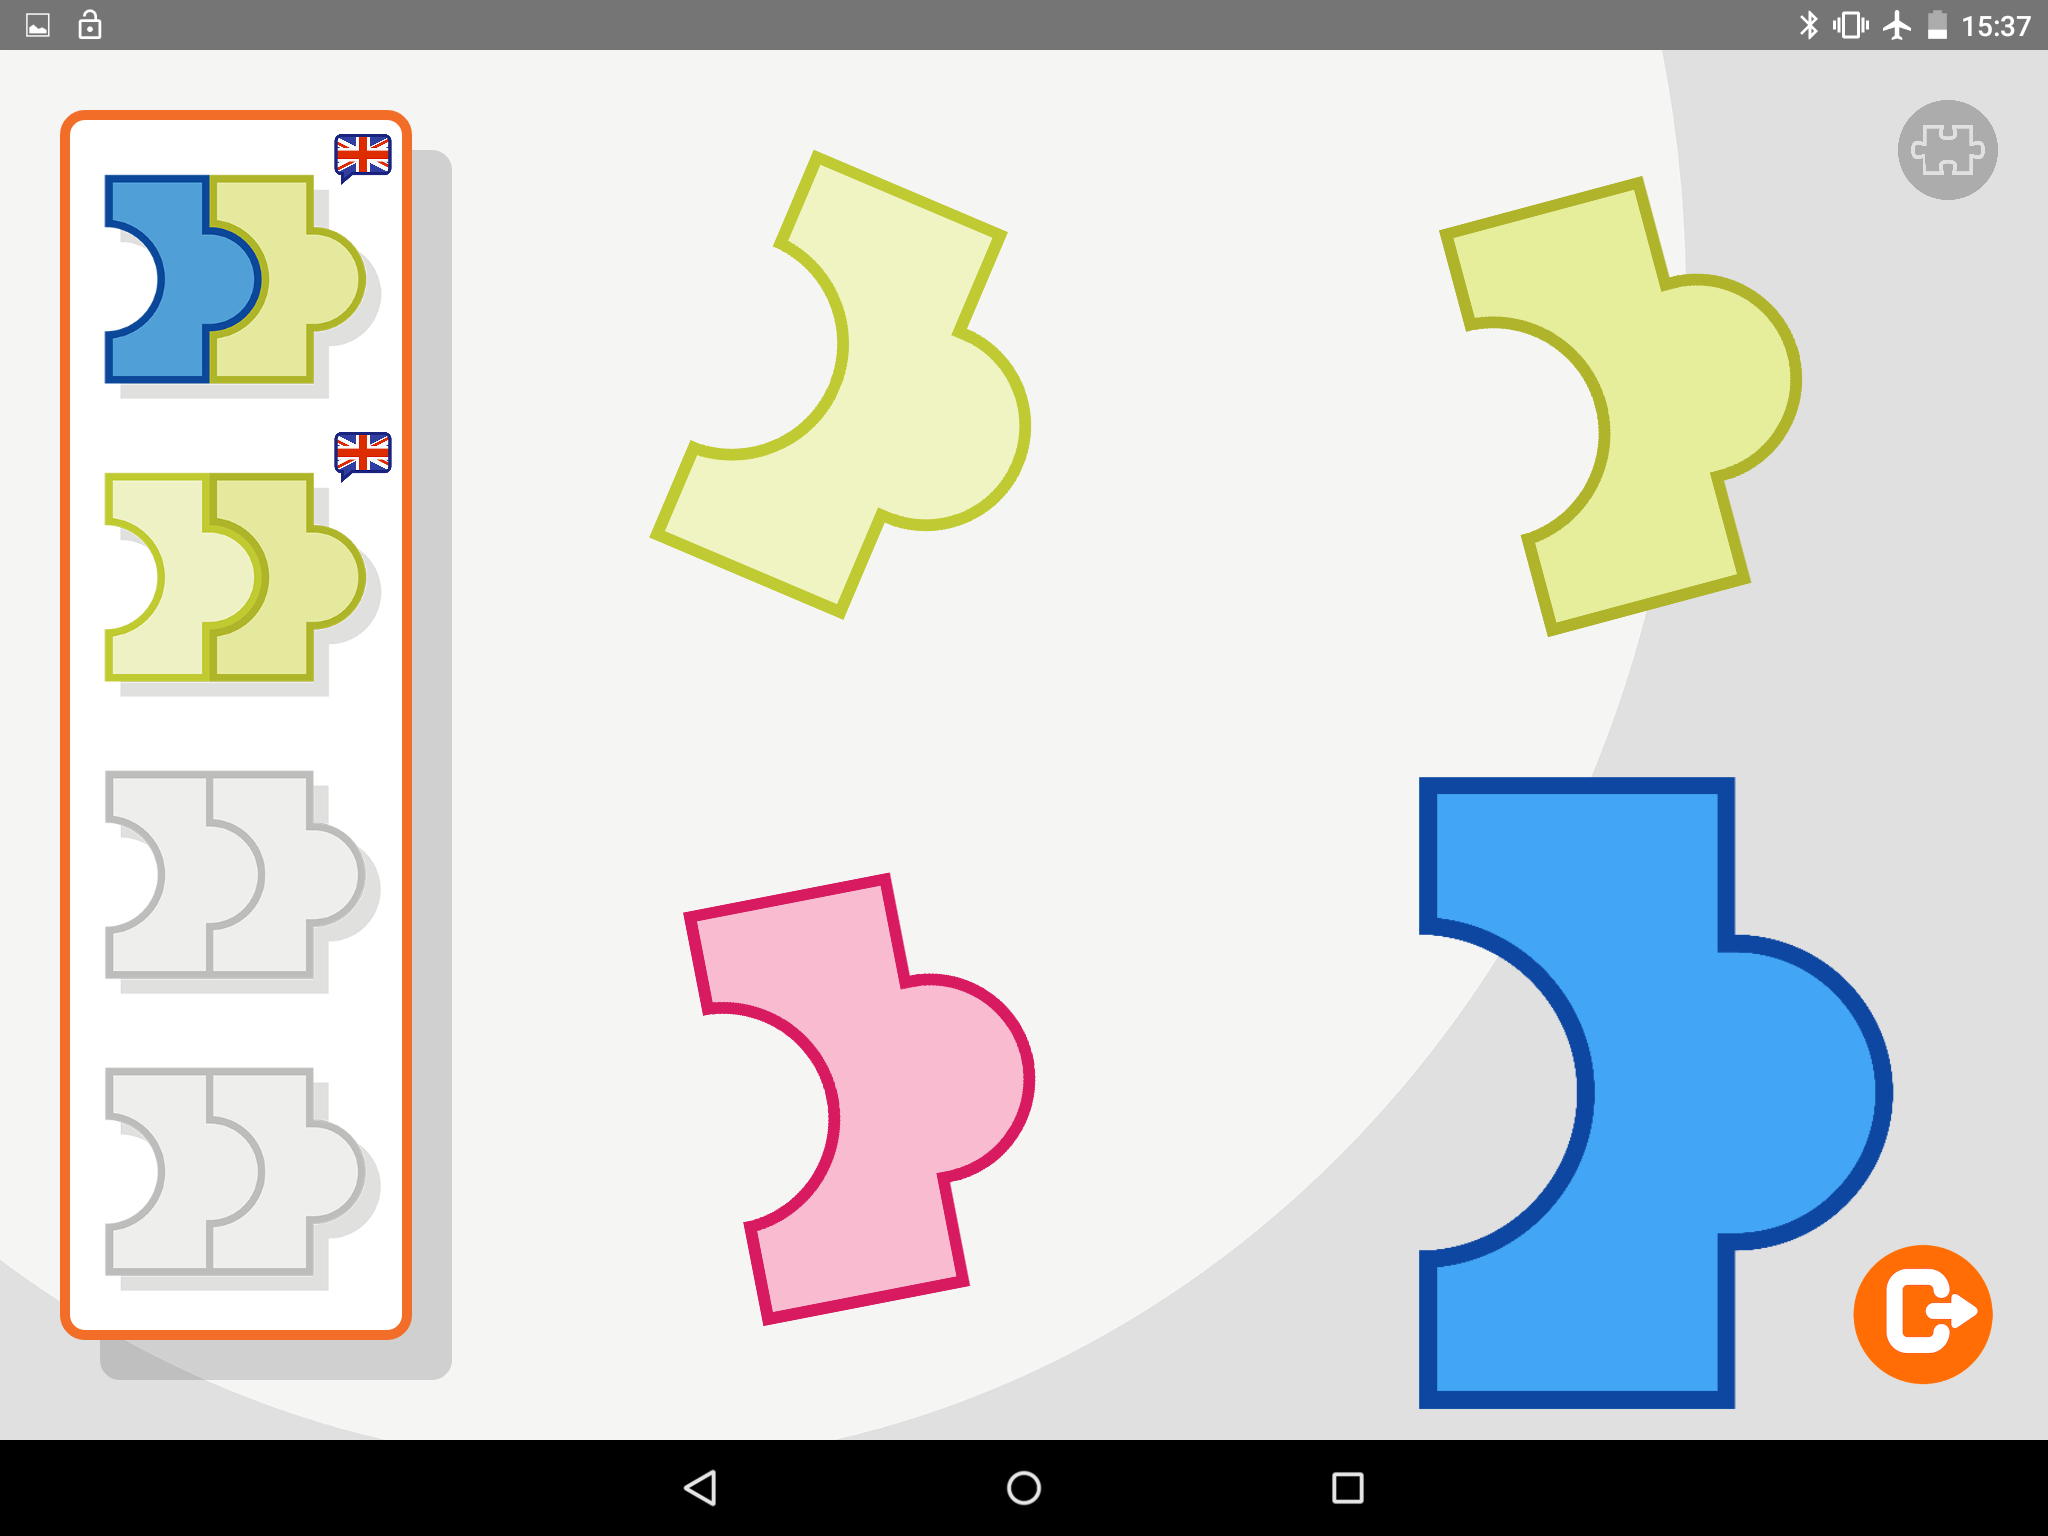
\includegraphics[width=\textwidth]{play_ui.png}}
  \caption{Schermata di gioco}
\end{figure}

%%--------------------------------------------------------------------------
%% DATABASE
%%--------------------------------------------------------------------------



\section{Database}

\subsection{Struttura}
\label{structure}
Il database SQLite è stato implementato tramite SugarORM, un ORM (Object-Relational Mapping) sviluppato appositamente per Android. In questo modo le entità del database sono direttamente mappate su classi Java, utilizzando il pattern DAO (Data Access Object).\\
Il database contiene 5 entità all'interno del package \\\code{it.gbresciani.legodigitalsonoro.model}:
\begin{description}
	\item[\code{Word}] Contiene la parola, sia in italiano sia in inglese, e le sillabe che lo compongono.
	\item[\code{Syllable}] Contiene la sillabla e l'esadecimale del colore associato.
	\item[\code{WordStat}] Permette di tracciare il momento in cui una parola viene trovata.
	\item[\code{GameStat}] Contiene le statistiche di una particolare partita
\end{description}
In figura \ref{fig:entities} sono riportati dettagli delle entità.

\begin{figure}[h!]
\label{fig:entities}
  \centering
    \centering{
      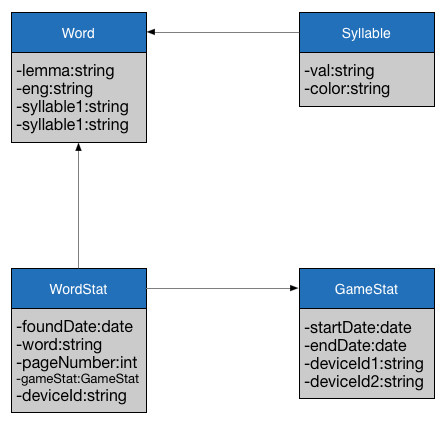
\includegraphics[width=\textwidth]{entities.png}}
  \caption{Entità presenti nel database}
\end{figure}

\subsection{Inizializzazione}
Il database viene inizializato la prima volta che l'applicazione viene aperta con i dati in formato \textit{JSON} presenti nei files \code{words.json} e \code{syllable.json} contenuti nella cartella degli \code{assets}.\\
Il listing \ref{lst:words_json} contiene un estratto del file \code{words.json}

\begin{lstlisting}[float, caption=Porzione del file \code{words.json}, label=lst:words_json]
[
  {
    "lemma":"arco",
    "eng":"arc",
    "syllable1":"ar",
    "syllable2":"co"
  },
  ...
\end{lstlisting}

Il mapping degli elementi JSON con la classe Java associata avviene tramite la libreria Open Source GSON, sviluppata da Goolge, che fa uso di annotazioni per mappare gli attributi delle classi con i campi JSON.\\
L'operazione di conversione dei dati da JSON a classi Java e il successivo inserimento all'interno del database, in quanto operazioni relativamente lunghe, non vengono eseguite all'interno del \textit{Thread} principale ma in uno differente grazie ad un \code{IntentService} contenuto in \\\code{it.gbresciani.legodigitalsonoro.services.InitDBService}. 


%%--------------------------------------------------------------------------
%% LOGICA DI GIOCO
%%--------------------------------------------------------------------------



\section{Logica di gioco}

\label{chap:game_logic}

La logica di gioco è affidata all'Activity \code{PlayActivity}; essa gestisce inoltre i \code{Fragments} (vedi capitolo \ref{chap:ui}) che visualizzano l'Intefaccia Utente.

\subsection{Glossario}
\label{sec:glossary}
In questa sezione vengono descritti acuni termini utili alla comprensione delle successive sezioni.

\begin{description}
\item[Page] Una partita è composta da una o più pagine. Una pagina può contenere 2 o 4 sillable e da 1 a 4 parole da trovare
\item[User role] Durante una partita multi player i giocatori si distinguono in ``master'', colui che ``orchestra'' la partita, e ``slave'', colui che vi partecipa in modo passivo 
\item[Turno] Durante una partita multi player rappresenta la possibilità per un giocatore di provare a indovinare una parola. Il giocatore che non è in possesso del turno attende la mossa dell'altro
\end{description}

\subsection{Event Bus}
\label{sec:event_bus}
Per far comunicare i vari componenti dell'applicazione (\code{Activities}, \code{Fragments}, \code{Services}) è stato utilizzato Otto, un \textit{Event Bus}, sviluppaato appositamente per Android, che permette ai vari componenti di postare eventi su un unico Bus e per riceverli in modo asincrono.\\
La classe \code{BusProvider} permette, tramite un metodo statico, di accedere allo stesso Bus in ogni punto dell'applicazione.\\
All'interno del package \code{package it.gbresciani.legodigitalsonoro.events} son presenti numerose classi (ad esempio \code{WordClickedEvent} o \code{PageCompletedEvent}) che rappresentano i diversi eventi generati e ``ascoltati'' dai componenti dell'app.\\
La classe \code{NineBus} è una piccola estensione del Bus predefinito di Otto che permette di pubblicare tutti gli eventi sul \code{Main Thread}, anche se generati in un altro \code{Thread}.

\subsection{GameState}
\label{sec:game_state}
\code{GameState} è la classe che rappresenta lo stato di una partita, sia essa single o multi player. Viene inizializzato da \code{PlayActivity}, e aggiornato durante il corso della partita in seguito ai diversi eventi prodotti dagli altri componenti dell'app.\\
I suoi attributi sono:
\begin{description}
    \item[pageNumber] Il numero di pagina corrente.
    \item[pages] Il numero di pagine totali della partita in corso (stabilito nelle impostazioni).
    \item[pageWordsToFindNum] Il numero di parole ancora da trovare nella pagina corrente.
    \item[wordsAvailable] Un \code{ArrayList} contentente le parole ancora da trovare.
    \item[wordsFound] Un \code{ArrayList} contenente le parole gia trovate.
    \item[syllables] Un \code{ArrayList} contenente le syllabe presenti nella pagina corrente.
    \item[currentPlayer] Se la partita è multi player contiene una stringa che rappresenta il ruolo del giocatore che detiene in quel momento il turno.
    \item[currentPlayerDeviceId] Se la partita è multi player contiene una stringa che rappresenta l'id del dispositivo che detiene in quel momento il turno.
\end{description}

La classe \code{GameState} contiene attributi annotati con \code{@SerializedName} in modo da poter essere convertita in un oggetto JSON (tramite GSON) ed essere inviata al secondo giocatore nel caso di partita multiplayer (maggiori dettagli nella sezione \ref{sec:multiplayer}).

\subsection{Statistiche di gioco}
\label{sec:stats}
Le satistiche della partita, come accennato nel capitolo sul database, vengono salvate tramite i DAO \code{WordStat} e \code{GameStat} che contengono, ad esempio, i tempi di ritrovamento delle parole, le parole stesse, la pagine su cui sono state trovate o eventualmente l'id del giocatore che le ha trovate.

\subsection{Game flow}
\label{sec:game_flow}
Tutta le fasi di una partita sono gestite dall'\code{Activity} \code{PlayActivity}.
All'avvio, cioè durante la chiamata al metodo \code{onCreate()} essa esegue le seguenti operazioni:
\begin{enumerate}
\item Carica i settaggi della partita
\item Carica i suoni di gioco
\item Istanzia il sintetizzatore vocale \code{TextToSpeech}
\item In base al tipo di partita (single o multi player) inizializza o meno il Bluetooth e setta la variabile \code{multi} a ``MASTER'' o ``SLAVE''
\end{enumerate}

I principali metodi di \code{PlayActivity} sono:
\begin{description}
\item[\code{startGame()}] Si occupa di inizializzare gli oggetti per le statistiche e chiama \code{constructPage()} and \code{startPage()}
\item[\code{constructPage()}] Inizializza lo stato della partita (\code{GameState}) con i dati relativi alla pagina corrente. Chiama i metodi accessori \code{Helper.chooseSyllables()} (sceglie in modo casuale le sillabe per la pagina) e \code{Helper.permuteSyllablesInWords()} (calcola le permutazione delle sillabe scelte per trovare le parole componibili)
\item[\code{startPage()}] Inizializza i \code{Fragments} che mostreranno l'interfaccia utente
\item[\code{updateState()}] Si occupa di gestire la logica di gioco: determina se tutte le parole sono state trovate o se interrompere il gioco quando non è il proprio turno e posta sul Bus l'evento \code{StateUpdatedEvent} in modo che i \code{Fragments} possano reagire correttamente
\end{description}

L'\code{Activity} presenta inoltre diversi metodi annotati con \code{@Subscribe} che permettono di reagire agli eventi pubblicati da altri componenti.

\subsection{Invio statistiche}
\label{sec:stats_send}
L'invio delle statistiche avviene tramite l'invio di una mail all'indirizzo settato nelle impostazioni dell'applicazione.\\
L'invio è gestito dall'\code{IntentService} \code{GenericIntentService} al quale viene passato l'id corrispondente alla partita appena conclusa. Interrogando il database esso carica i dati e li inserisce nel corpo dell'email formattandoli come mostrato nel listing \ref{lst:stats}. Il listing \ref{lst:stats_example} ne mostra invece un esempio.

\begin{lstlisting}[float, caption=Struttura delle satistiche inviate, label=lst:stats]
Dispositivo N: device id
Tempo totale: mm:ss
N - word: mm:ss (# of page on which the word was found)
...
\end{lstlisting}


\begin{lstlisting}[float, caption=Esempio di statistiche, label=lst:stats_example]
- One player -

Dispositivo 1: BC:20:A4:73:6B:49
Tempo totale: 00:13
1 - fumo: 00:02 (1)
1 - muro: 00:13 (2)

- Two Player -

Dispositivo 1: BC:20:A4:73:6B:49
Dispositivo 2: D4:0B:1A:15:FD:AD
Tempo totale: 00:14
2 - ceno: 00:02 (1)
1 - noce: 00:09 (1)
2 - buco: 00:14 (2)
\end{lstlisting}

\subsection{Multiplayer}
\label{sec:multiplayer}
Come già detto la modalità multi player segue le stesse regole di quella single player se non per il fatto che i due giocatori provano a turno a trovare una parola.\\
Il tablet ``master'' è quello che inizia il processo di connessione scegliendo, tra i dispositivi in ascolto, il tablet ``slave''. I vari aspetti della partita come i settaggi, le sillabe presenti e le parole da trovare vengono tutti stabiliti dal ``master'' che si occupa quindi anche di gestire il flow del gioco, mentre lo ``slave'' partecipa in modo passivo.\\
La comunicazione tra i due dispositivi avviene tramite Bluetooth. La classe che si occupa di stabilire la connessione è \code{BluetoothService}; essa si serve di tre \code{Thread} differenti (\code{AcceptThread}, \code{ConnectThread}, \code{ConnectedThread}) per ricevere un connessione, effettuare una connessione, e inviare e ricevere messaggi.\\
I messaggi scambiati sono stringhe contenenti oggetti JSON preceduti da un header che ne identifica la natura. I possibili messaggi sono $4$:

\begin{description}
    \item[GAME\_STATE] Contiene la rappresentazione JSON dell'oggetto \code{GameState} descritto nella sezione \ref{sec:game_state}. Solo il ``master'' invia questo tipo di messaggio allo ``slave'', il quale ne ricava tutte le informazioni necessarie.
    \item[SIMPLE\_TURN\_PASS] Lo ``slave'' invia questo messaggio al ``master'' quando non è riuscito a trovare parole e quindi sta semplicemente passando il turno.
    \item[WORD\_FOUND] Lo ``slave'' invia questo messaggio insieme alla parola trovata, in modo che il ``master'' possa aggiornare lo stato della partita.
    \item[GAME\_END] Il ``master'' invia questo messaggio allo ``slave'' al termine della partita.
\end{description}

%%--------------------------------------------------------------------------
%% INTERFACCIA UTENTE
%%--------------------------------------------------------------------------



\section{User Interface}
\label{chap:ui}

Come anticipato nel capitolo \ref{chap:game_logic}, l'interfaccia grafica del gioco è gestita quasi interamente da \code{Fragments}, che rispondono agli eventi pubblicati sul Bus dall'activity \code{PlayActivity} aggiornando i loro componenti.\\
I due principali \code{Fragments} sono \code{WordsFragment} e \code{SyllablesFragment} (vedi figura \ref{fig:fragments}), che si occupano rispettivamente di gestire la porzione di schermo contenente le parole, e la porzione contenente le sillabe disponibili.

\begin{figure}[h!]
\label{fig:fragments}
  \centering
    \centering{
      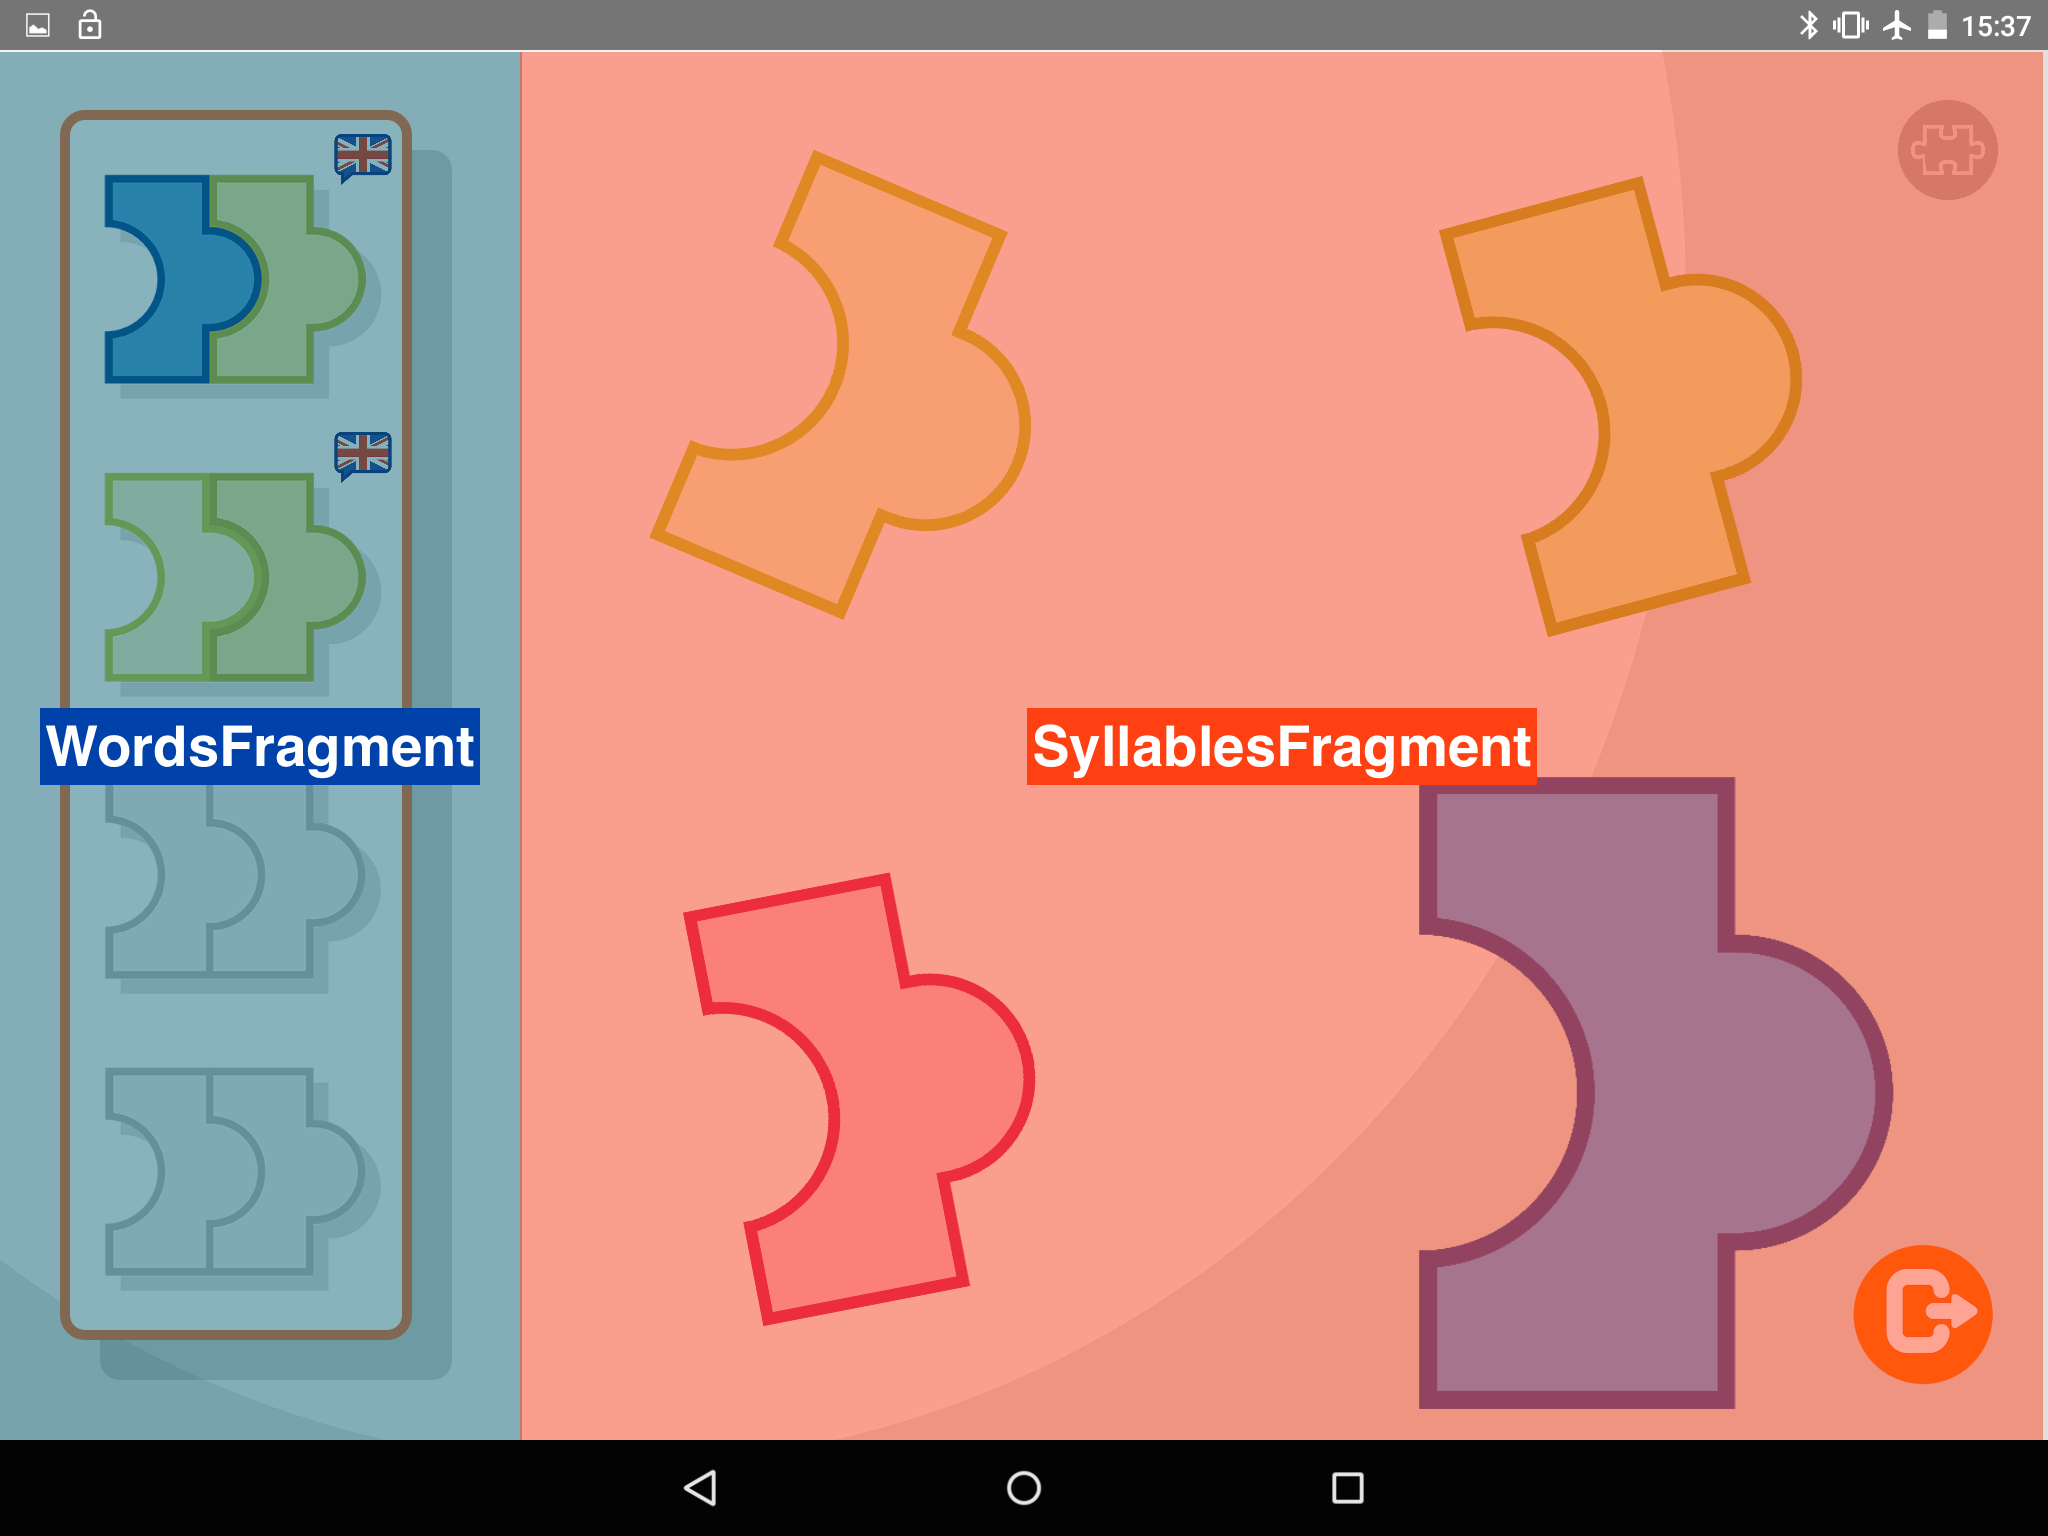
\includegraphics[width=\textwidth]{fragments.png}}
  \caption{Fragments della schermata di gioco}
\end{figure}


\subsection{WordsFragment}
\label{sec:words_fragment}
\code{WordsFragment} si occupa di gestire la parte di interfaccia grafica che rigurda le parole già trovate e quella ancora da trovare.\\
Esso presenta una lista verticale di ``slot'' che possono essere ``vuoti'', o ``riempiti'' con le tessere di puzzle corrispondenti alle sillabe che formano la parola. Viene inoltre mostrata accanto ad ogni slot ``pieno'' una bandiera inglese che se toccata permette di ascolare il suono della parola tradotta in inglese.\\
Il metodo \code{initUI()} si occupa, dato il numero di parole da trovare e la dimensione dello schermo (calcolata a runtime), di calcolare la dimensione degli slot corretta per gli slot con lo scompo di riempire al meglio lo spazio disponibile.\\
Le immagini degli slot sono fornite come file PNG all'interno della cartella \code{assets} e vengono caricate dinamicamente come Bitmap della dimensione corretta (per risparimare memoria) dal metodo \code{loadWordBitmap()}.\\
Il \code{Fragment} è sottoscritto all'evento \code{StateUpdatedEvent} in modo da reagire ai cambiamenti di stato della partita, come il ritrovamento di una nuova parola.

\subsection{SyllablesFragment}
\label{sec:syllables_fragment}

\code{SyllablesFragment} si occupa di gestire la parte di interfaccia grafica che rigurda le sillabe disponibili nella pagina corrente.\\
Esso presenta una griglia sparsa di 2 o 4 tessere di puzzle colorate rappresentanti ognuna una sillaba. Se toccate le tessere vengono selezionate e si ``alzano'' per restituire un feedback della selezione e riproducono il suono della sillaba a cui sono associate.\\
Al pari di \code{WordsFragment} calcola la dimensione corretta delle immagini e le carica come Bitmap.

%%--------------------------------------------------------------------------
%% LIBRERIE
%%--------------------------------------------------------------------------



\subsection{Librerie esterne}
Di seguito vengono elencate le librerie utilizzate per lo sviluppo dell'applicazione.

\begin{description}

\item[\href{http://satyan.github.io/sugar}{SugarORM}] \hfill \\
Libreria Open Source ORM.

\item[\href{https://code.google.com/p/google-gson/}{Gson}] \hfill \\
Libreria Java che permette la conversione tra oggetti Java e la loro rappresentazione JSON.

\item[\href{http://square.github.io/otto/}{Otto}] \hfill \\
Libreria che permette di sfruttare un event bus.

\item[\href{https://github.com/JakeWharton/butterknife}{ButterKnife}] \hfill \\
Libreria per l'injection delle View.
\end{description}


\section{Manuale Utente}
%%--------------------------------------------------------------------------
%% MANUALE UTENTE
%%--------------------------------------------------------------------------

Dalla schermata principale (figura \ref{fig:lego2_main}), toccando l'icona grigia in alto a sinistra dello schermo, si può accedere alla schermata delle impostazioni (figura \ref{fig:lego2_settings}) da cui si possono impostare i parametri di gioco e l'indirizzo e-mail per l'invio dei dati.

\screenshot{lego2_main}{La schermata principale}
\screenshot{lego2_settings}{La schermata di impostazioni}

Sempre dalla schermata iniziale si può dare inizio al gioco sia in modalità multi-giocatore, che singolo. Se si sceglie la prima, allora si verrà rimandati alla schermata di associazione tramite \textit{bluetooth} (figura \ref{fig:lego2_multi}).

\screenshot{lego2_multi}{La schermata di associazione tramite \textit{bluetooth}}

Una volta iniziata la partita (figura \ref{fig:lego2_game}), si potrà giocare cliccando sulle sillabe fino al suo termine.

\screenshot{lego2_game}{La schermata di gioco}



\chapter{Trova l'Intruso 1}
\renewcommand*{\mypath}{trovaintruso1}%
\graphicspath{ {\mypath/images/} }

\doctitle{Paolo Ferraris}{paolo2.ferraris@mail.polimi.it}
\localtoc

\section{Descrizione delle classi}

\noindent Per prima cosa vengono descritte le classi principali, partendo dal modello che definisce il gioco, in seguito vengono descritte le classi Helper che permettono la gestione della logica, e infine le Activity utilizzate.

\subsection{Classi del modello dati}

\noindent Di seguito sono descritte le classi che gestiscono il modello del gioco, rappresentate nel class diagram della Figura \ref{fig:class_diagram}:

\begin{figure}
	\centering
	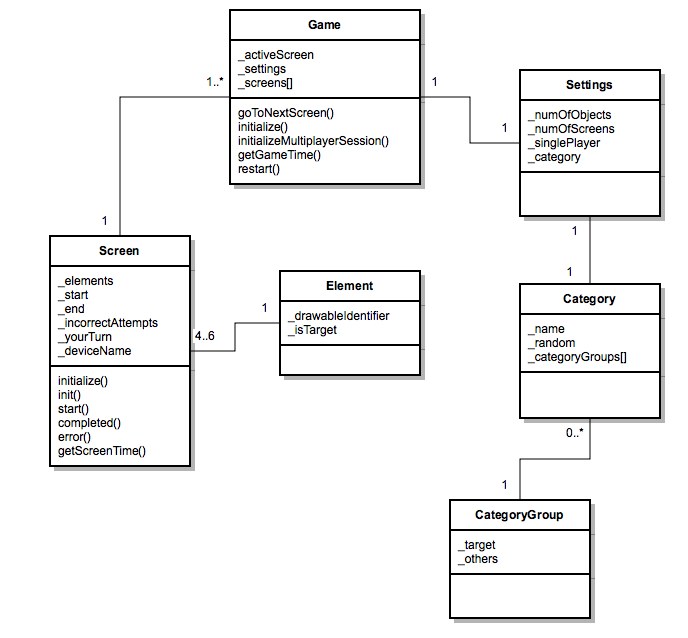
\includegraphics[width=13.5cm]{trova_l_intruso_class_diagram}
	\caption{Class Diagram}
	\label{fig:class_diagram}
\end{figure}
\begin{description}
\item \textbf{Game} \`{e} la classe che gestisce la partita, i principali metodi sono:
\begin{itemize}
\item initialize(): metodo che inizializza la sessione di gioco, creando i livelli e assegnandone gli oggetti da visualizzare.
\item initializeMultiplayerSession(boolean guest): metodo che stabilisce i turni di gioco nelle partite multiplayer, la variabile guest indica se il dispositivo \`{e} quello che \`{e} stato invitato a giocare.
\item goToNextScreen(): metodo che attiva la schermata successiva e restituisce true. Nel caso ci si trovi nell'ultimo livello restituisce false.
\item fillScreens(): riempie le schermate con le immagini in base alla categoria e al numero di oggetti da visualizzare.
\item CreateGameDescription(Context context): crea la descrizione della partita da mandare via mail.
\item restart(): riavvia il gioco con le stesse impostazioni.
\end{itemize}
\item \textbf{Settings} Classe che gestisce le impostazioni di gioco, possiede le seguenti propriet\`{a}:
\begin{itemize}
\item \_singlePlayer(Boolean): indica la modalit\`{a} di gioco.
\item \_numOfObjects(int): indica il numero di immagini visualizzate per livello.
\item \_numOfScreens(int): indica il numero di livelli impostati.
\item \_category(Category): indica la categoria di immagini selezionata.
\end{itemize}

\item \textbf{Screen}
Classe che rappresenta il livello di gioco, possiede come propeirt\`{a} il tempo di inzio livello, il tempo di fine, una variabile booleana che indica se \`{e} il turno del giocatore corrente, il numero di errori e un array contenente le immagini da visualizzare. I principali metodi sono:
\begin{itemize}
\item initialize(): inizializza il livello, inserendo le immagini.
\item init(): azzera le variabili del livello, ossia numero di errori, tempo di gioco.
\item start(): avvia il gioco su questo livello, settando la variabile \_start\_time.
\item error(): incrementa il conteggio degli errori di uno.
\item completed(): metodo evocato quando il livello \`{e} completato, setta la variabile \_end\_time.
\item getScreenTime(): restituisce il tempo di gioco.
\end{itemize}
\item \textbf{Element}
\noindent Classe che rappresenta un immagine, possiede due attributi, il nome dell'immagine presente nella cartella \emph{drawable} e un valore booleano che indica se \`{e} l'elemento target.
\item \textbf{Category}
Classe che rappresenta una categoria di immagini, possiede come propriet\`{a} il nome della categoria, un campo booleano che indica se si tratta di una categoria "Casuale" e una lista di oggetti CategoryGroups relativi alla categoria. Il costruttore accetta un JSONObject contenente la definizione della categoria e da esso inizializza l'oggetto.
\item \textbf{CategoryGroup}
Classe che rappresenta una gruppo di immagini che deve essere rappresentato in una schermata. Definisce l'elemento target e i restanti elementi.
\end{description}

\subsection{Classi Helper}

\begin{description}
\item \textbf{CategoryHelper} Gestisce il caricamento delle categorie di immagini dal file .json dove sono definite.
\item \textbf{GameHelper} Gestisce le meccaniche di gioco e la comunicazione tra i dispositivi in multiplayer. I principali metodi di questa classe sono:
\begin{itemize}
\item onMainActivityCreate(): metodo utilizzato all'avvio dell'activity principale, avvia il riconoscimento dei dispositivi sul network (per le partite in multiplayer) e carica le impostazioni di gioco precedentemente salvate.
\item onMainActivityDestroy(): chiamato quando l'activity principale viene distrutta, viene terminato il servizio di discovery sul network e viene chiusa la connessione (se attiva).
\item registerCurrentActivity(Activity activity): metodo chiamato nell'onCreate di ogni activity, registra l'activity mostrata a schermo per gestire al meglio le comunicazioni tra i dispositivi in multiplayer e la visualizzazione di avvisi o dei feedback di gioco.
\item startGame(): Questo metodo inizializza il gioco, viene chiamato il metodo Game.initialize() e in seguito se il gioco \`{e} in SinglePlayer viene caricata l'activity Screen nella quale viene mostrato il primo livello, altrimenti si passa all'activity MultiPlayerDiscoveryActivity per invitare un giocatore.
\item quitGame(): questo metodo serve per terminare una partita, e nel caso di partite multiplayer viene chiusa anche la connessione.
\item nextScreen(): metodo che serve per passare al livello successivo, in caso di partite multiplayer viene inviato l'analogo messaggio all'altro dispositivo.
\end{itemize}
\item \textbf{MultiPlayerServiceHelper} Gestisce il riconoscimento dei dispositivi che eseguono il gioco sulla rete per permettere l'avvio di partite multiplayer.
\item \textbf{ConnectionHelper} Il multiplayer \`{e} implementato usando i socket Java, questa classe gestisce la connessione, l'invio di messaggi sul network e inizializza gli oggetti ServerHelper e ClientHelper.
\item \textbf{ServerHelper} Gestisce il lato server della connessione, avviando un SocketServer thread che si occupa dell'assegnamento di una connessione al socket client appena arriva una richiesta al server.
\item \textbf{ClientHelper} Questa classe istanzia due thread, un thread che si occupa della ricezione dei messaggi in arrivo al socket utilizzato per la connessione, e uno che si occupa di inviare i messaggi al dispositivo col quale si sta giocando.
\end{description}

\subsection{Gestione della comunicazione in partite multiplayer}
\noindent Per la gestione delle comunicazioni tra dispositivi nelle partite multiplayer \`{e} stata creata una classe GameMessage, la quale definisce una propriet\`{a} di tipo Serializable, che rappresenta il contenuto del messaggio, e una propriet\`{a} chiamata "Type", un enum che indica il tipo di messaggio, che pu\`{o} assumere i seguenti valori:
\begin{itemize}
\item \emph{ConnectionRequest}: i messaggi di questo tipo non hanno contenuto e servono ad inoltrare a un dispositivo una richiesta di connessione per avviare una partita;
\item \emph{ConncectionAccepted}: questo messaggio viene inviato dal client al server quando il giocatore accetta di giocare;
\item \emph{ConncectionClosed}: questo messaggio viene inviato prima di chiudere la connessione;
\item \emph{SendGame}: con questo messaggio viene inviata la struttura del gioco al dispositivo invitato a giocare;
\item \emph{SendGameAck}: questo messaggio conferma la ricezione del messaggio precedente da parte del client;
\item \emph{StartGame}: questo messaggio viene inviato al dispositivo client per comunicargli di avviare il gioco, alla sua ricezione il client avvia il gioco e manda il messaggio di ack al server;
\item \emph{StartGameAck}: questo messaggio conferma la ricezione del messaggio precedente, alla sua ricezione il dispositivo server a sua volta avvia il gioco;
\item \emph{ElementPressed}: con questo messaggio viene inviato l'indice dell'elemento premuto all'altro dispositivo in modo da visualizzare il feedback;
\item \emph{NextScreen}: con questo messaggio si comunica al dispositivo avversario che il giocatore ha premuto il pulsante per cambiare schermata.
\end{itemize}

\subsection{Activity}

\noindent Di seguito vengono descritte le principali Activity presenti nell'app:

\begin{description}
\item \textbf{MainActivity}: \`{e} l'activity che si presenta all'avvio del gioco, inizializza la propriet\`{a} globale GameHelper e permette di avviare il gioco.
\item \textbf{ScreenActivity}: l'activity che gestisce il livello di gioco, all'avvio vengono caricate le immagini e mostrate a schermo, in seguito si attende l'input dell'utente e si visualizzano a schermo i feedback.
\item \textbf{ResultsActivity}: l'activity che viene mostrata alla fine del gioco, mostra i risultati dei livelli e permette di riavviare il gioco oppure tornare alla MainActivity.
\item \textbf{MultiPlayerDiscoveryActivity}: in questa activity vengono mostrati gli altri giocatori e si pu\`{o} iniziare una partita multiplayer.
\item \textbf{SettingsActivity} e \textbf{ConfigDeviceActivity} permettono la configurazione delle impostazioni della partita e del dispositivo.
\end{description}

\section{Modello della sessione di gioco}

\noindent
Nella Figura \ref{fig:activity_diagram} \`{e} riportato l'activity diagram che schematizza lo svolgimento del gioco.

\begin{figure}
	\centering
    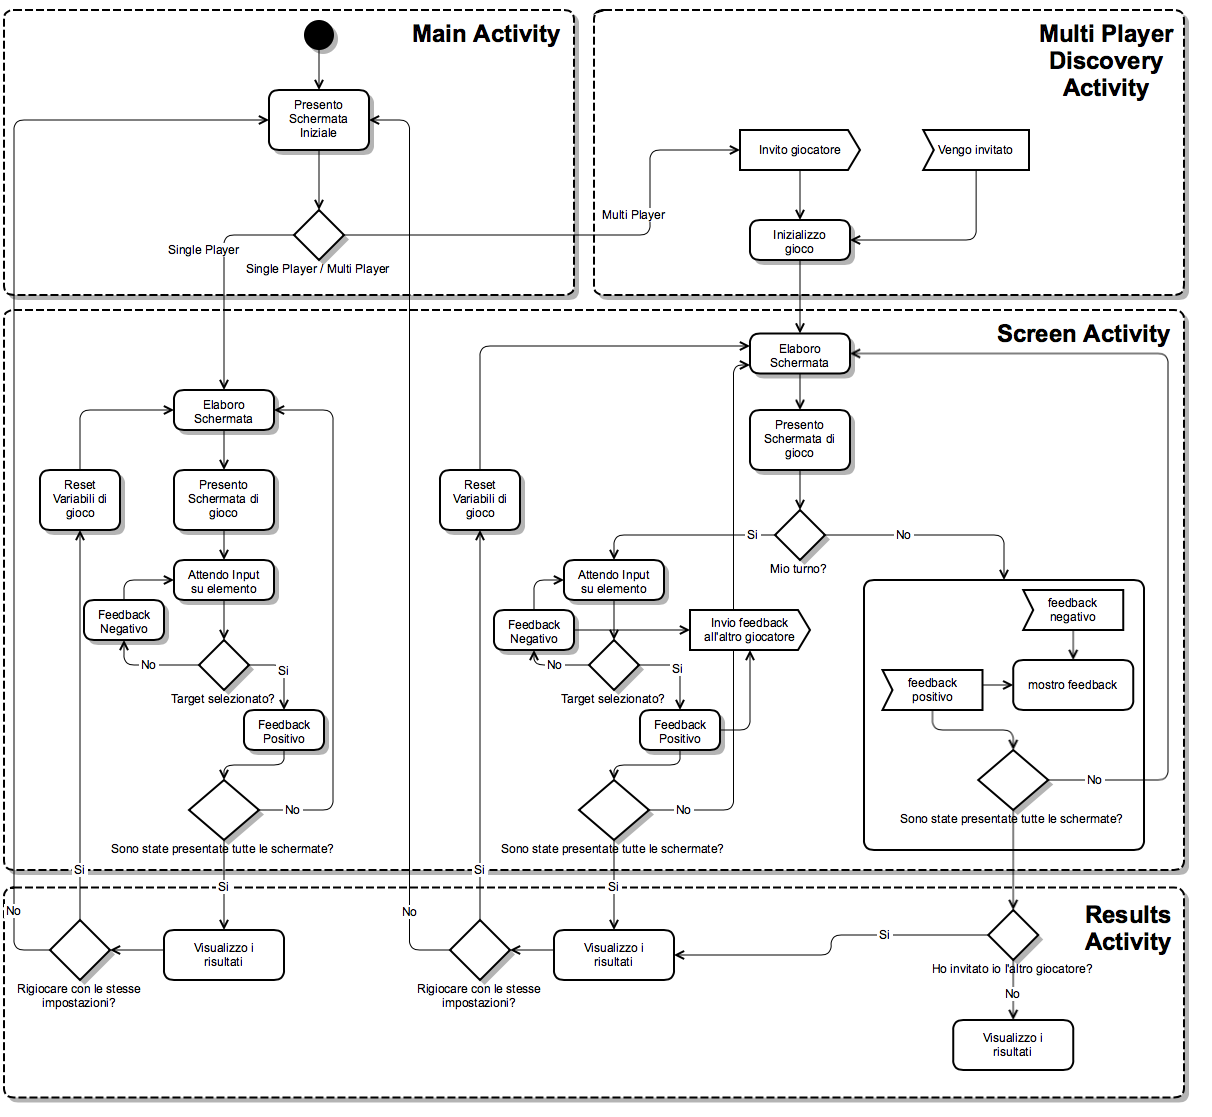
\includegraphics[width=13.5cm]{trova_l_intruso_android}
	\caption{Class Diagram}
	\label{fig:activity_diagram}
\end{figure}

%\subsection{Inizializzazione di una partita mutliplayer}

%\noindent Il sequence diagram


\chapter{Trova l'Intruso 2}
\renewcommand*{\mypath}{trovaintruso2}%

\doctitle{Riccardo Medana}{r.medana@gmail.com}
\localtoc

\graphicspath{ {\mypath/images/} }

\section{Manuale Sviluppatore}
\subsection{Descrizione delle classi}
Vengono descritte di seguito le classi principali, iniziando da quelle che costituiscono il modello dati. Successivamente vengono descritte le classi utility che permettono la gestione di elementi comuni alle varie parti dell'app, infine le Activity che compongono l'applicazione.

\subsubsection{Classi del modello dati}
Il modello dati del gioco è rappresentato in figura \ref{fig:class}.

\begin{figure}[h!]
\centering{
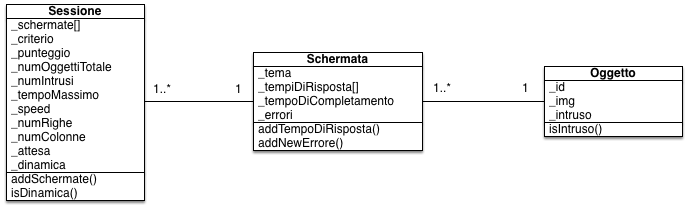
\includegraphics[width=\textwidth]{class.png}}
\caption{Class Diagram del modello dati}
\label{fig:class}
\end{figure}

\begin{itemize}
\item \textbf{Oggetto} è la classe che rappresenta il singolo oggetto sullo stage di gioco.
\item \textbf{Schermata} è la classe che rappresenta la singola schermata di gioco. Una schermata contiene da 1 a N oggetti (N è definito in base alla modalità di gioco)
\item \textbf{Sessione} è la classe che rappresenta l'intera sessione di gioco. Una sessione è costituita da una o più schermate.
\end{itemize}

Tutte le classi sopracitate, oltre ai metodi particolari riportati nello schema, espongono anche i relativi metodi getter e setter per accedere agli attributi.
\subsubsection{Classi utility}

\begin{itemize}
\item \code{DbAdapter} e \code{DatabaseHelper} sono due classi che contengono i metodi per la gestione del database delle email (le email da inviare al termine della partita vengono salvate in una tabella che agisce da coda di invio, per ogni email viene salvato il testo e l'indirizzo email di destinazione).
\item \code{GmailSender} è la classe che contiene la logica per poter inviare il report della sessione di gioco via mail. Questa classe utilizza la classe \code{JSSEProvider} per gestire l'autenticazione nella connessione al server di posta in uscita.
\item \code{ImgUtils} contiene alcuni metodi per la gestione delle immagini all'interno del gioco
\item \code{JsonUtils} contiene i metodi per accedere alle strutture dati JSON che definiscono le possibili schermate (v. Strutture Dati)
\item \code{MailUtils} contiene il metodo che spedisce la mail in modalità asincrona, assieme al metodo che compone il messaggio da spedire
\item \code{TimeUtils} contiene il metodo che scrive il tempo in secondi in una stringa nel formato corretto.
\item \code{ViewContainer} e \code{ViewContainerAccessor} sono due classi predefinite per la gestione delle animazioni con la libreria Universal Tween Engine, definiscono il contenitore per la view da animare e il modo in cui dev'essere animata.
\end{itemize}

\subsubsection{Activity}

\begin{itemize}
\item \code{MainActivity} è l'activity presentata all'avvio dell'app, propone le due modalità di gioco e il setup.
\item \code{SetupActivity} è l'activity che consente di modificare i parametri di gioco.
\item \code{ModeOneActivity} è l'activity che esegue la modalità di gioco dinamica (con oggetti in movimento)
\item \code{ModeTwoActivity} è l'activity che esegue la modalità di gioco statica (griglia con oggetti fissi nello spazio)
\end{itemize}

La descrizione dei singoli metodi contenuti nelle activity è riportata all'interno del codice.

\subsection{Strutture dati}
All'interno della cartella \code{Assets} sono riportati alcuni file JSON che descrivono le possibili schermate per ogni criterio (forma, percettivo, colore). Ad esempio, il file \code{percettivo.json}:

\begin{lstlisting}[float, caption=Contenuto del file \code{percettivo.json}, label=lst:percettivo_json]
{
    "scene" : [
        {
                 "id" : "universo",
                 "nome" : "Universo",
                 "target" : "stella",
                 "elementi" : [
                        {"nome" : "pianeta_1"},
                        {"nome" : "pianeta_2"},
                        {"nome" : "pianeta_3"}
                 ],
                 "sfondo" : "bg_universo"
        },
        {
                   "id" : "prato",
                   "nome" : "Prato",
                   "target" : "quadrifoglio",
                   "elementi" : [
                          {"nome" : "trifoglio"}
                   ],
                   "sfondo" : "bg_prato"
        },
        {
                 "id" : "natura",
                 "nome" : "Natura",
                 "target" : "tartaruga",
                 "elementi" : [
                        {"nome" : "anguria"}
                 ],
                 "sfondo" : "bg_prato"
        }
    ]
}
\end{lstlisting}

Per ogni scena vengono specificati quali sono gli elementi grafici da utilizzare per comporla.

\subsection{Modello della sessione di gioco}
Nella figura \ref{fig:session} è riportato il flusso di gioco, con riferimento alle attività contenute nelle activity.

\begin{figure}[h!]
\centering{
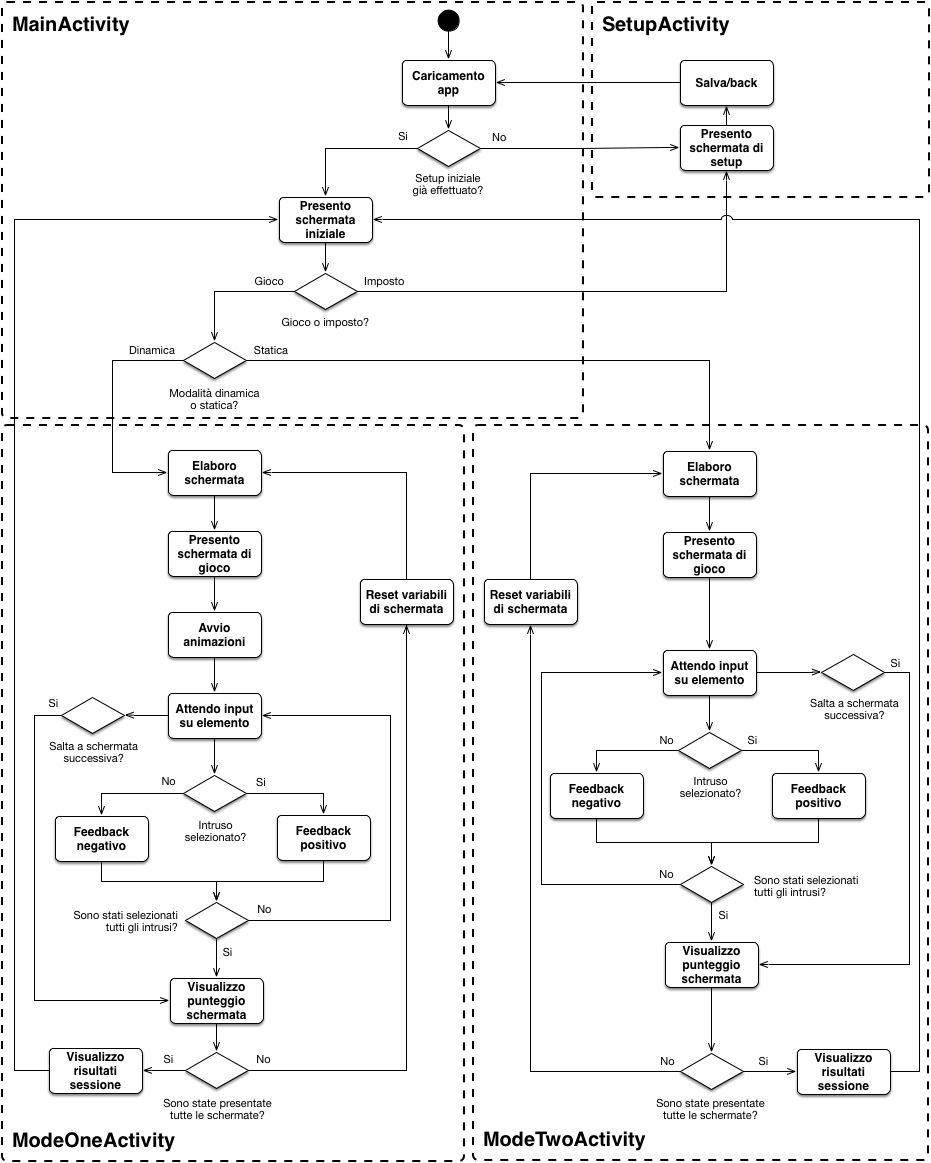
\includegraphics[width=\textwidth]{session.png}}
\caption{Modello della sessione di gioco}
\label{fig:session}
\end{figure}


\section{Manuale Utente}
\subsection{Primo avvio}
Al primo avvio del gioco viene richiesto di effettuare il setup con i parametri necessari a giocare. Specificare quindi gli indirizzi email per l'invio e la ricezione dei report di gioco, assieme ai parametri di gioco. Premere “Salva impostazioni” per tornare alla schermata iniziale. Fino a quando non vengono salvate le impostazioni non è possibile cominciare a giocare.

\subsection{Impostazioni di gioco}
Per accedere alle impostazioni di gioco toccare l'icona grigia in alto a sinistra nella schermata iniziale.

\subsubsection{Impostazioni e-mail}
Per l'invio della mail è necessario un account Gmail. Nel caso in cui si dovessero riscontrare problemi con l'invio della mail è necessario abilitare l'accesso ad app meno sicure andando qui: \url{https://www.google.com/settings/security/lesssecureapps}
I messaggi inviati dall'app saranno disponibili nella cartella Posta Inviata dell'account Gmail utilizzato.
La mail viene inviata solo se il selettore “Invio mail al termine della sessione di gioco” è posizionato su ON, se è attiva la connessione a Internet e solo se sono state visualizzate tutte le schermate (anche saltandole nel corso del gioco).
La mail viene inviata dopo la comparsa della finestra “Partita terminata”, premendo sul pulsante di uscita.
Nel caso in cui i dati di accesso a Gmail fossero errati, o non fosse presente una connessione a Internet attiva al termine della partita, viene mostrato un messaggio di errore. La mail in questo caso non viene persa, ma salvata in una coda di invio. Le mail da spedire vengono inviate al termine della prima partita in cui la connessione a Internet è attiva e se i dati di accesso a Gmail sono corretti.

\subsubsection{Impostazioni modalità con oggetti in movimento}
In questa modalità il bambino deve individuare gli oggetti intrusi nascosti in un gruppo di oggetti in movimento. 
Occorre specificare:

\begin{itemize}
\item Email di destinazione dati (può essere anche un indirizzo email non Gmail)
\item Criterio di gioco (forma/colore/percettivo)
\item Numero di schermate da giocare
\item Numero totale di oggetti sullo schermo (non più di 50, inclusi gli intrusi)
\item Numero di intrusi nel gruppo di oggetti (in numero inferiore al totale degli oggetti)
\item Tempo massimo di gioco per schermata (in secondi)
\end{itemize}

\subsubsection{Impostazioni modalità con oggetti fissi nello spazio}
In questa modalità il bambino deve individuare gli oggetti intrusi nascosti in una griglia di oggetti. Gli intrusi appaiono e scompaiono nel corso della partita, occorre toccarli prima che scompaiano. 
Occorre specificare:

\begin{itemize}
\item Email di destinazione dati (può essere anche un indirizzo email non Gmail)
\item Criterio di gioco (forma/colore/percettivo)
\item Numero di schermate da giocare
\item Numero di righe (non più di 6)
\item Numero di colonne (non più di 10)
\item Numero di intrusi (in numero inferiore al totale degli oggetti)
\item Tempo massimo di gioco per schermata (in secondi)
\item Tempo di attesa prima che compaia l'intruso (in secondi)
\item Tempo di esposizione dell'intruso sullo schermo (in secondi)
\end{itemize}



\chapter{SuperApp}
\renewcommand*{\mypath}{superapp}%
\graphicspath{ {\mypath/images/} }

\doctitle{Lorenzo Affetti}{lorenzo.affetti@polimi.it}
\localtoc


\section{Introduzione}
Lo scopo dell'applicazione quello di mettere in atto una collaborazione tra quattro giocatori attraverso diverse modalità di gioco.
Ogni giocatore della squadra gioca su un tablet diverso, uno \textit{slave}. Il gioco necessita di un ulteriore tablet, il \textit{master}, che non verrà utilizzato da nessun giocatore, ma che fornirà informazioni di massima sulla partita in corso e scandirà le partite e le manche di gioco.

I dispositivi comunicano per mezzo di una connessione \textit{Bluetooth}. Un disegno di massima delle posizioni dei tablet è fornito in figura \ref{fig:tablet5}.

\begin{figure}[h!]
\centering{
\includegraphics[width=\textwidth]{tablets.png}}
\caption{I cinque tablet}
\label{fig:tablet5}
\end{figure}

L'applicazione comprende tre diversi giochi:

\begin{itemize}
\item \textit{Trova l'Intruso}: I giocatori devono, appunto, trovare l'intruso. Ad un certo numero di risposte esatte consecutive (configurabile) la logica di gioco si inverte (vengono dati feedback sonori e visivi) e il gioco diventa, quindi, trova il \textit{non} intruso. Questo gioco può essere lanciato in quattro diverse modalità: trova l'intruso per colore, \textit{ancora-colore} (come la modalità per colore, con la differenza che le immagini vengono mostrate in bianco e nero all'inversione di gioco), direzione e forma. 
\item \textit{Ordina dal Più Piccolo al Più Grande}: I giocatori devono ordinare quattro oggetti dal più piccolo al più grande o viceversa.
\item \textit{Costruisci la Torre}: I giocatori devono completare una torre composta da quattro oggetti giocando a turno.
\end{itemize}

In ognuno dei tre giochi l'applicazione sottopone agli utenti delle immagini che si muovono con velocità variabile su dei nastri trasportatori.

Ogni \textit{partita} è composta da un numero di \textit{manche} (o \textit{stage}) configurabile. Il completamento di tutte le manche porta alla vittoria del gruppo. I punteggi sono sempre cumulativi dell'intera squadra.

\section{Struttura Generale}
% - i vari pattern di comunicazione
% TODO diagramma di interazione back <-> front (con tanto di eventi)

\begin{figure}[h!]
\centering{
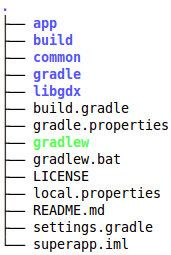
\includegraphics[height=7cm,keepaspectratio]{tree_root.png}}
\caption{La struttura del progetto (profondità 1)}
\label{fig:tree_root}
\end{figure}

Il codice sorgente dell'applicazione è suddiviso in tre moduli (figura \ref{fig:tree_root}). Il modulo \code{app} contiene il backend, comprensivo di logica di gioco e di comunicazione, e il frontend dell'applicazione. Il modulo \code{libgdx} contiene le parti più interattive dell'applicazione e cioè quelle dei nastri trasportatori. Infine, il modulo \code{common} contiene moduli privi di dipendenze dal framework di Android e usati in ambedue i precedenti moduli.

Come già accennato, SuperApp è divisa in tre diversi giochi di cui il primo è disponibile in quattro modalità diverse (in realtà, anche il secondo, tuttavia la logica di gioco rimane invariata tra di esse, ciò che varia è solo l'ordinamento delle quattro immagini iniziali). Per questo motivo, quasi ogni classe costituente il nucleo della logica di gioco (si veda sezione \ref{subsec:logic}) e diversi \textit{fragment} (si veda sezione \ref{subsec:activities}) segue il particolare schema di ereditarietà illustrato in figura \ref{fig:hierarchy}, a parte sporadiche eccezioni che, però, sono facilmente comprensibili a una prima lettura del codice (per esempio, abbiamo \code{Slave1Color} e \code{Slave1ColorAgain}, ma solo un \code{MasterColor} poiché il ruolo del \textit{master} nelle due modalità non cambia).

\begin{figure}[h!]
\centering{
\includegraphics[width=\textwidth]{hierarchy.png}}
\caption{Lo schema di ereditarietà generale}
\label{fig:hierarchy}
\end{figure}

Gli elementi costitutivi dell'intera applicazione sono:

\begin{description}
\item[i \textit{Controller}] rappresentano la logica di gioco e mantengono il suo stato;
\item[i \textit{Tile}] o tesserini, costituiscono il modello dell'applicazione (si veda la classe \code{it.playfellas.superapp.tiles.Tile} nel modulo \code{common}). Sono le immagini che l'utente toccherà per dare delle risposte;
\item[la \textit{UI}] mostra il gioco all'utente e raccoglie le sue azioni;
\item[i \textit{Presenter}] interpretano le azioni dell'utente fornite dalla \textit{UI} fornendole ai \textit{Controller}. In base al responso ottenuto, vanno a informare la \textit{UI} dei cambiamenti da apportare.
\item[il \textit{Bus}] permette la comunicazione per mezzo di \textit{eventi} tra gli elementi costitutivi dell'applicazione (in locale) e tra i dispositivi coinvolti (in remoto, tramite \textit{Bluetooth}). Per maggiori informazioni riguardo alla comunicazione, si veda la sezione \ref{subsec:tenbus}.
\end{description}

Il diagramma in figura \ref{fig:components} mostra i vari componenti di SuperApp e la loro interazione ad alto livello su un dispositivo \textit{slave}. Il diagramma fornito non vuole essere esaustivo di tutti i possibili messaggi scambiati tra i moduli, bensì vuole chiarire le idee al lettore e fornire un'idea di massima delle interazioni tra le classi.

\begin{figure}[h!]
\centering{
\includegraphics[width=\textwidth]{components.png}}
\caption{Le componenti di SuperApp su uno \textit{slave}}
\label{fig:components}
\end{figure}


\section{Backend}

\subsection{Il TenBus}
\label{subsec:tenbus}
Prima di spiegare il funzionamento di qualsiasi altro componente di SuperApp è necessario introdurre il \code{TenBus}, parte del package \code{it.playfellas.superapp.network}. Questa classe è quella che permette a tutte le componenti del sistema di comunicare tra di loro -- sia in remoto che in locale -- per mezzo della trasmissione di \textit{eventi}. Il \code{TenBus} è un \textit{wrapper} attorno al \textit{bus} ad eventi \textbf{Otto} (\url{http://square.github.io/otto/}).

Dopo aver ottenuto un'istanza del \code{TenBus} tramite il metodo statico \code{get}, un oggetto può \code{post}are \code{NetEvent} oppure \code{InternalEvent}. I primi verranno inviati in remoto sul canale \textit{Bluetooth}, i secondi verranno propagati in locale usando l'originale Otto. Gli eventi sono di molteplici tipi e le loro classi sono contenute nel package \code{it.playfellas.superapp.events}, la loro generazione è accentrata nella \code{EventFactory}.

Se un oggetto volesse ricevere degli eventi, dovrà semplicemente invocare il metodo \code{register} passando un qualsiasi oggetto (anche \code{this}) che abbia registrato dei metodi tramite l'annotazione \code{@Subscribe}. I methodi annotati devono accettare in ingresso un oggetto di tipo uguale all'evento interessato e ritornare un valore \code{void}.

Il \code{TenBus} offre anche i metodi \code{attach} e \code{detach} per permettere lo scambio di eventi in remoto. Per il funzionamento dettagliato della connessione \textit{Bluetooth} (inizializzazione, chiusura) si veda il codice.

Le classi \code{BTThread} e \code{Peer} (e quelle che le estendono) sono volutamente invisibili all'esterno del package \code{network}, l'unico punto d'accesso alla rete per un oggetto esterno è il \code{TenBus}.

\subsection{La Logica di Gioco}
\label{subsec:logic}
% la GameHistory?

\begin{figure}[h!]
\centering{
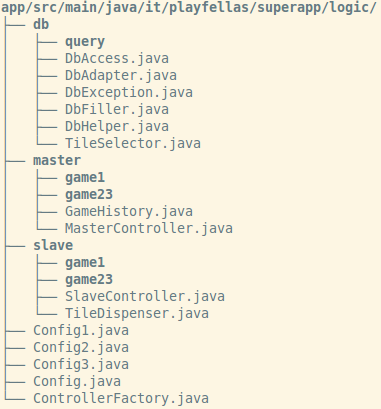
\includegraphics[height=10cm,keepaspectratio]{tree_logic.png}}
\caption{La struttura del package \texttt{it.playfellas.superapp.logic}}
\label{fig:tree_logic}
\end{figure}

Gli elementi fondamentali della logica di gioco sono contenuti nel package \code{it.playfellas.superapp.logic} (per una struttura del package si veda figura \ref{fig:tree_logic}):

\begin{description}
\item[\textbf{I Dispenser}]\hfill\\
    Sostanzialmente sono, come chiarisce la \textit{signature} della classe \code{it.playfellas.superapp.logic.slave.TileDispenser}, degli \code{Iterator<Tile>}. Quello che un \textit{dispenser} fa, infatti, è fornire un nuovo \textit{tile} ad ogni invocazione del metodo \code{next}. Ogni modalità di gioco ha un suo particolare \textit{dispenser} (il gioco 1 ne ha, invece, due: uno normale e l'altro per l'inversione di gioco), il quale interroga il \textit{database} dell'applicazione (che contiene solo \textit{tile}) per ottenere un insieme di tesserini. Questi ultimi verranno forniti ai \textit{controller} tramite il metodo \code{next} secondo logiche proprie del \textit{dispenser} stesso. Per indagare le logiche specifiche si veda il codice sorgente degli specifici \code{TileDispenser} contenuti nei package \code{it.playfella.superapp.logic.slave.game1} e \code{game23};
\item[\textbf{I Master Controller}]\hfill\\
    I \textit{controller} rappresentano la logica di logico. Ogni azione che l'utente compie per mezzo di un gesto sullo schermo del tablet viene interpretata dalla parte di \textit{UI} e viene passata ad un \textit{controller} che saprà interpretarla e fornire una risposta in base allo stato attuale della partita. I \textit{master}, nello specifico, sono quelli che mantengono lo stato globale della partita (per esempio: il punteggio, i giocatori, ecc.) e danno inizio alle partite sugli \textit{slave} (si veda il metodo \code{beginStage}) fornendo, a volte, informazioni condivise (per esempio, nel gioco 1, il colore/forma/direzione base; nei giochi 2 e 3, le quattro \textit{tile} di base). Oltre a dare inizio alle partite, ne scandiscono ogni fase, come il loro inizio e la loro fine e l'inizio e la fine delle manche che le compongono.
\item[\textbf{Gli Slave Controller}]\hfill\\
    Gli \textit{slave} attendono che i \textit{master} trasmettano gli eventi di inizio/fine partita e inizio/fine manche per poter dare inizio al gioco vero e proprio. Essi istanziano i \textit{dispenser} per ottenere i prossimi \textit{tile} da fornire agli utenti e contengono anche la parte di logica di gioco riguardante l'esattezza o meno di un \textit{tile} date le sue caratteristiche (vedi metodo \code{isTileRight}). Quest'ultima informazione è quella che verrà trasmessa tramite eventi al \textit{master} che deciderà, di conseguenza, se incrementare o azzerare (o altro) il punteggio complessivo. Ogni \code{SlaveController} fornisce anche il metodo \code{nextTile}, il quale \textit{delega} ad un \textit{dispenser} l'ottenimento del prossimo \textit{tile} (metodo \code{next}) da mostrare all'utente. Sarà poi la parte di \textit{UI} che mostrerà il tesserino all'utente posizionandolo nel momento giusto sul nastro trasportatore usando il \code{DisposingService} (si veda \code{it.playfellas.superapp.ui.slave}).
\end{description}

\subsubsection{La Partita}
Come precedentemente detto, la partita è articolata in un numero configurable di stage. Ognuno di essi prevede un punteggio massimo configurabile. Al raggiungimento di tale punteggio, lo stage termina e si dà inizio allo stage successivo. Quando tutti gli stage sono stati completati, la partita finisce.

La scansione della partita nelle suddette fasi è determinata dal \code{MasterController}. Esso invia, tramite il \code{TenBus}, un evento \code{StartGameEvent} (in realtà, viene inviato un evento che estende quella classe. Per esempio: \code{StartGame1Color}, oppure \code{StartGame2Event}, ecc.). Alla ricezione dell'evento, ogni \textit{slave} reagisce mostrando la schermata di gioco all'utente. A questo punto, il \textit{master} procede per stage fino al loro esaurimento: viene inviato un \code{BeginStageEvent} e lo stage ha inizio; quando il punteggio massimo viene raggiunto, il \textit{master} invia un \code{EndStageEvent} seguito da un ulteriore \code{BeginStageEvent} in caso vi sia un altro stage da giocare, altrimenti viene inviato un \code{EndGameEvent}.

In figura \ref{fig:game_flow}, viene rappresentata la successione di eventi che regolano lo svolgimento della partita.

\begin{figure}[h!]
\centering{
\includegraphics[width=\textwidth]{game_flow.png}}
\caption{La partita}
\label{fig:game_flow}

\end{figure}

\subsection{L'invio dei Dati di Gioco}
Per l'invio dei dati abbiamo utilizzato il \textit{database} non relazionale di \textbf{Firebase} (\url{https://www.firebase.com/docs/android/quickstart.html}).

La classe \code{GameHistory} si prende carico di memorizzare tutte le azioni intraprese dai giocatori e il loro esito, tramite l'esposizione dei metodi \code{right} e \code{wrong}. Sarà il \code{MasterController} a invocare questi metodi della \code{GameHistory} dopo aver ricevuto i \code{RWEvent} da parte degli \textit{slave}. Alla fine della partita, il \textit{master} persiste i dati sul \textit{backend} \textit{Firebase}.

La disponibilità di connettività internet non è comunque necessaria proprio grazie al funzionamento interno di \textit{Firebase}: i dati verranno infatti salvati nel suo \textit{database} locale fino a che la connettività sarà disponibile, in quel momento, i dati verranno salvati nel \textit{database} remoto.

La struttura dai dati è quella di un oggetto \textit{JSON}. I dati in remoto, infatti, possono essere esportati come file \code{.json} in qualsiasi momento.

Il dato di una partita contiene il suo \textit{ID} (visibile sulla schermata di gioco del \textit{master}), la sua storia completa (ogni singolo \textit{click} da parte dei giocatori e l'esattezza o meno della risposta data) e più di dieci indici. La struttura del dato è ancora da considerarsi variabile fino a sperimentazione conclusa.

Riportiamo un esempio di dato per una partita, troncato dove la struttura dei dati è ripetitiva e dove l'informazione è ridondante, nel listato \ref{lst:data}.

\begin{lstlisting}[
    basicstyle=\linespread{1}\ttfamily,
    caption=Un esempio di dato per una partita,
    label=lst:data
]
{
  "dd42247e" : {
    "history" : [ {
      "deltaT" : 0.0,
      "player" : "player4",
      "rw" : false,
      "ts" : "28/09/2015 13:34:06:074"
    }, {
      "deltaT" : 0.001,
      "player" : "player3",
      "rw" : true,
      "ts" : "28/09/2015 13:34:06:075"
    },
            // more and more clicks ...
    ],
    "index10_noRightPerPlayer" : {
      "player_player1" : 10,
      "player_player2" : 7,
      "player_player3" : 11,
      "player_player4" : 11
    },
    "index11_noWrongPerPlayerPerStage" : {
      "player_player1" : {
        "stage_1" : 8,
        "stage_2" : 3,
        "stage_3" : 3,
        "stage_4" : 1
      },
            // more players ...
    },
    "index12_noWrongPerPlayer" : {
        // hidden
    },
    "index13_ratio9_11" : {
        // hidden
    },
    "index14_ratio10_12" : {
        // hidden
    },
    "index15_clicksRatio" : {
        // hidden
    },
    "index1_elapsedTime" : 9.166666666666666E-4, // very low because it was auto-generated
    "index2_noWrongPerStage" : {
      "stage_1" : 24,
      "stage_2" : 12,
      "stage_3" : 13,
      "stage_4" : 12
    },
    "index3_noWrong" : 61,
    "index4_noRightPerStage" : {
        // hidden
    },
    "index5_noRight" : 39,
    "index6_playerContributionPerStage" : {
      "player_player1" : {
        "stage_1" : {
          "1-3" : 0.23076923076923078,
          "2-3" : 0.46153846153846156,
          "3-3" : 0.35714285714285715
        },
                // more stages...
      },
                // more players...
    },
    "index7_balancePerStage" : {
      "stage_1" : {
        "1-3" : 5.25,
        "2-3" : 7.25,
        "3-3" : 3.5
      },
            // more stages...
    },
    "index8_playerContributionStabilityPerStage" : {
        // hidden
    },
    "index9_noRightPerPlayerPerStage" : {
        // hidden
    }
  }
}
\end{lstlisting}

I dati sono salvati all'indirizzo \url{https://giocoso2015.firebaseio.com/}. Per le credenziali di accesso, si contatti \url{lorenzo.affetti@polimi.it}.

\section{Frontend}

\subsection{Le Activity e i Fragment}
\label{subsec:activities}
In questa sezione riportiamo un elenco delle \textit{activity} e dei \textit{fragment} e le loro principali mansioni.
Per il codice sorgente si faccia riferimento al package \code{it.playfellas.superapp.ui}.

\newcommand{\includescreenshot}[2]{
\begin{figure}[h!]
\centering{
\includegraphics[width=\textwidth]{screenshots/#1.png}}
\caption{#2}
\label{fig:#1}
\end{figure}
}

\begin{description}
\item[MainActivity (fig. \ref{fig:master_slave})]\hfill\\
    è il punto di accesso dell'applicazione, permette di scegliere tra \textit{master} e \textit{slave};

\includescreenshot{master_slave}{La \code{MainActivity}}

\item[master.MasterActivity (fig. \ref{fig:master_gameselection})]\hfill\\
    permette la scelta tra i diversi giochi (1, 2 e 3);

\includescreenshot{master_gameselection}{La selezione del gioco}

\item[master.GameActivity]\hfill\\
    è l'\textit{activity} in cui avviene la partita nel \textit{master}. Contiene i seguenti \textit{fragment}:

    \begin{description}
    \item[SettingsFragment (fig. \ref{fig:master_gamesettings})]\hfill\\
        permette di configurare il gioco corrente;

    \includescreenshot{master_gamesettings}{Il \textit{master} configura la partita che sta per iniziare}

    \item[GameFragment (fig. \ref{fig:master_game})]\hfill\\
        mostra lo stato della partita (stage, punteggio, foto dei giocatori, ecc.). Istanzia il giusto (per la modalità di gioco corrente) \code{GamePresenter} che a sua volta istanzia il giusto \code{MasterController}.

    \includescreenshot{master_game}{La schermata che mostra lo stato della partita sul \textit{master}}
    \end{description}

\item[master.bluetooth.BluetoothActivity (fig. \ref{fig:master_btactivity})]\hfill\\
    permette l'associazione dei dispositivi.

\includescreenshot{master_btactivity}{La connessione \textit{master}/\textit{slave} tramite \textit{Bluetooth}}

\item[master.bluetooth.FastStartActivity (fig. \ref{fig:master_faststart})]\hfill\\
    permette l'avvio rapido del \textit{master} riassociando gli ultimi dispositivi connessi.

\includescreenshot{master_faststart}{La schermata di configurazione veloce di gioco}

\item[slave.SlaveActivity (fig. \ref{fig:slave_waiting})]\hfill\\
    \textit{activity} in cui lo \textit{slave} aspetta di venir scelto dal \textit{master} come giocatore della partita tramite associazione \textit{Bluetooth};

    \includescreenshot{slave_waiting}{La schermata di attesa di connessione per lo \textit{slave}}

\item[slave.GameActivity]\hfill\\
    è l'\textit{activity} in cui avviene la partita nello \textit{slave}. Tramite la ricezione degli eventi che estendono \code{StartGameEvent}, determina la modalità di gioco corrente e sceglie, di conseguenza, il giusto \textit{fragment} da mostrare. Contiene i seguenti \textit{fragment}:

    \begin{description}
    \item[PhotoFragment (fig. \ref{fig:slave_photo})]\hfill\\
        l'utente può scattarsi una foto da utilizzare come \textit{avatar} durante la partita;

    \includescreenshot{slave_photo}{Lo scatto della foto dell'utente}

    \item[SlaveGameFragment (fig. \ref{fig:slave_game1}, \ref{fig:slave_game2} e \ref{fig:slave_game3})]\hfill\\
        contiene i nastri trasportatori e i \textit{tiles} (vedi sezione \ref{subsec:libgdx}). Istanzia i nastri trasportatori e il giusto \code{SlavePresenter} (che istanzia il giusto \code{SlaveController}) in base alla modalità di gioco corrente.

    \includescreenshot{slave_game1}{La schermata di gioco nel gioco 1}
    \includescreenshot{slave_game2}{La schermata di gioco nel gioco 2}
    \includescreenshot{slave_game3}{La schermata di gioco nel gioco 3}
    \end{description}
\end{description}

Per l'istanziazione dei \textit{controller} si faccia riferimento a \code{it.playfellas.superapp.logic.ControllerFactory}.

\subsection{I Nastri}
\label{subsec:libgdx}
Il modulo del progetto che gestisce la visualizzazione e lo scorrimento dei nastri e la rappresentazione e animazione dei \textit{tile} è \code{libgdx}. \textbf{LibGDX} (\url{https://libgdx.badlogicgames.com/features.html}) è un framework Java che utilizza \textbf{OpenGL} (\url{https://www.opengl.org/}) per la renderizzazione video. Il risultato della scelta di questo framework è un miglioramento sia nella fluidità delle animazioni, che nell'occupazione della memoria del dispositivo da parte dell'applicazione rispetto all'utilizzo dell'\code{ObjectAnimator} standard di Android.

\textit{LibGDX} racchiude i concetti più comuni dei framework di renderizzazione grafica. Troviamo infatti la \textit{scena}, il ``luogo''in cui avvengono le animazioni, e gli \textit{sprite}, immagini bidimensionali dotate di posizione, \textit{texture} (la loro immagine), altezza e larghezza.

Gli elementi costitutivi del modulo \code{libgdx} sono:

\begin{description}
    \item[la Scene] la \textit{scena} del gioco;
    \item[i Conveyor] i nastri trasportatori su cui vengono posati i \textit{tile}. Essi possono essere di diversi tipi. Troviamo infatti \code{MovingConveyor} (figura \ref{fig:movingconveyor}), \code{SizeConveyor} (figura \ref{fig:sizeconveyor}) e \code{TowerConveyor} (figura \ref{fig:towerconveyor}).\\
        Bisogna notare che gli ultimi due non sono propriamente nastri trasportatori in quanto sono statici. Essi vengono utilizzati nei giochi 2 e 3 rispettivamente.

    \includescreenshot{movingconveyor}{Un nastro trasportatore}
    \includescreenshot{sizeconveyor}{Il ``nastro trasportatore''statico del gioco 2}
    \includescreenshot{towerconveyor}{Il ``nastro trasportatore''statico del gioco 3}

    \item[le TileRepr] dei \textit{wrapper} intorno ad un \code{Tile} e un \code{SimpleSprite}. Essi sono la rappresentazione concreta di un \textit{Tile} (quello del modello dell'applicazione). La corrispondenza \code{TileRepr} (rappresentazione), \code{Tile} (modello) è talmente stretta e semanticamente equivalente che, da ora in poi, utilizzeremo i due termini in modo intercambiabile.
\end{description}

Ciò che avviene ad ogni frame di visualizzazione è l'esecuzione del metodo \code{render} della \code{Scene}, il quale aggiunge ogni \textit{sprite} presente nella scena ad un \textit{batch} di renderizzazione, dopo averne aggiornato posizioni, texture e dimensioni. Il \textit{batch} così generato, contenente una matrice di pixel che rappresenta il ``disegno''degli \textit{sprite} aggiunti, viene renderizzato tramite l'invocazione di \code{batch.end()}.

Per comprendere cosa si intende per ``aggiornamento''di uno \textit{sprite}, si pensi alla sua posizione: per far muovere un nastro o un \textit{tile}, infatti, è necessario cambiare la sua posizione pixel per pixel ad ogni frame di rappresentazione (si vedano i metodi \code{update} nelle classi che estendono \code{Conveyor}).



\end{document}
